% =====================================================================
%  Chapter 4 — Fertility trends in the post-Soviet space, 2000–2023
%  Input with:  % =====================================================================
%  Chapter 4 — Fertility trends in the post-Soviet space, 2000–2023
%  Input with:  % =====================================================================
%  Chapter 4 — Fertility trends in the post-Soviet space, 2000–2023
%  Input with:  % =====================================================================
%  Chapter 4 — Fertility trends in the post-Soviet space, 2000–2023
%  Input with:  \input{chapters/04_trends}
%  Requires: \input or \include of tables/tab_country_tfr.tex, and the
%  four PNG figures in figures/.
% =====================================================================

\section{Fertility Trends in the Post-Soviet Space, 2000--2023}
\label{sec:trends}

\subsection{Levels and trajectories}
\label{sec:levels}

In 2000 the fourteen countries in this study ranged from 1.11 children per woman in Ukraine to 3.49 in Tajikistan. Twenty-three years later the range had not narrowed. Ukraine had fallen to 0.98, one of the lowest national fertility rates ever recorded anywhere, while Uzbekistan had risen to 3.50. The endpoints are almost identical to where they started; what changed is which countries occupy them and how they got there.

\input{tables/tab_country_tfr}

Table~\ref{tab:country-tfr} sets out the individual trajectories, and Figure~\ref{fig:all-countries} shows all fourteen together. Two things stand out immediately. The first is the separation. In every single year of the panel, the lowest-fertility Central Asian country lies above the highest-fertility country outside Central Asia. There is not one crossing in twenty-four years, and the narrowest the two groups ever come is 0.195 children per woman, in 2012.

\begin{figure}[htbp]
  \centering
  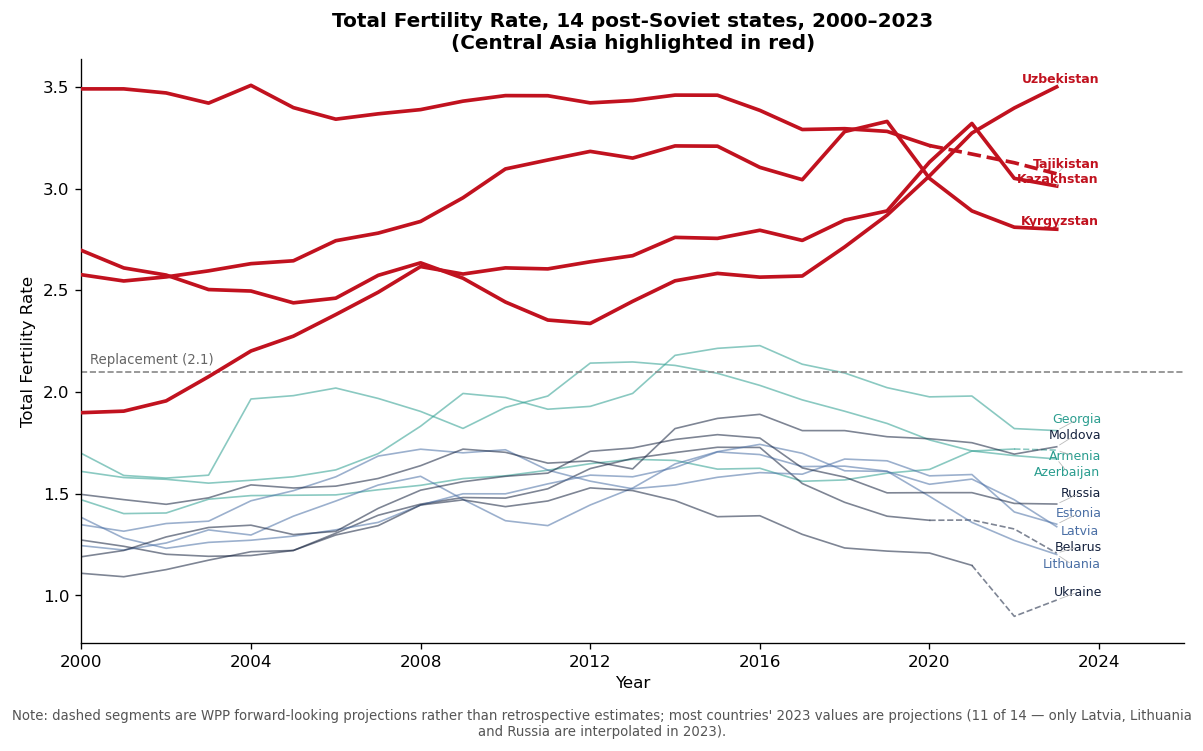
\includegraphics[width=\textwidth]{figures/fig1_all_countries}
  \caption{Total fertility rate, fourteen post-Soviet states, 2000--2023. Central Asian countries in red. Dashed segments are WPP forward-looking projections rather than retrospective estimates.}
  \label{fig:all-countries}
\end{figure}

The second is that the separation does not come from a shared decline at different speeds. Most of the sample rose for the first fifteen years or so. Ten of the fourteen countries recorded their highest fertility of the period in 2015 or later, and only Tajikistan among the Central Asian states peaked early, in 2004. Russia's rate climbed from 1.19 to a high of 1.79 in 2015 before falling back; Latvia went from 1.24 to 1.74 in 2016; Georgia reached 2.23 in 2016, briefly above replacement. This broad recovery from the post-Soviet trough is well documented for the European successor states \parencite{billingsley2010,grigoras2019} and for Central Asia \parencite{spoorenberg2015}. What has not been documented, because the comparative literature ends before it, is what happened after that.

By 2023 ten of the fourteen countries were below the replacement level of 2.1, and the four that were not are the four Central Asian states. Three of the ten European and Caucasian countries had fallen below 1.25.

\subsection{The difference between the blocs}
\label{sec:gap}

Figure~\ref{fig:bloc-means} tracks the two bloc means with the country range around each. The Central Asian mean rose from 2.67 in 2000 to 3.09 in 2023, an increase of 0.43 children per woman. The rest of the post-Soviet space rose too, from 1.38 to a peak of 1.77 in 2016, and then gave nearly all of it back, ending at 1.44.

\begin{figure}[htbp]
  \centering
  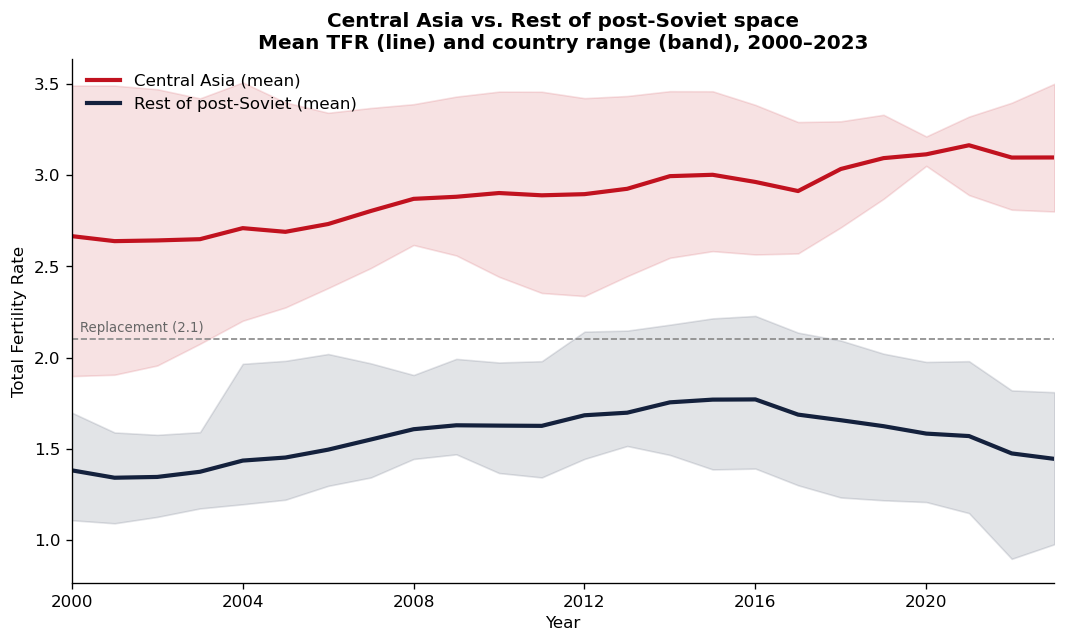
\includegraphics[width=0.92\textwidth]{figures/fig2_bloc_means}
  \caption{Mean total fertility rate by bloc, with the country range shown as a shaded band, 2000--2023.}
  \label{fig:bloc-means}
\end{figure}

The difference between the two means is the central descriptive object of this thesis, and its behaviour over time is more interesting than its average size. Figure~\ref{fig:gap} plots it year by year. From 2000 to 2016 it is remarkably flat, moving within a narrow corridor between 1.19 and 1.30 and drifting very slightly downward. Then it changes character: 1.19 in 2016, 1.38 in 2018, 1.53 in 2020, 1.65 in 2023. Over seven years it widened by 0.46 children per woman, having barely moved in the previous sixteen.

\begin{figure}[htbp]
  \centering
  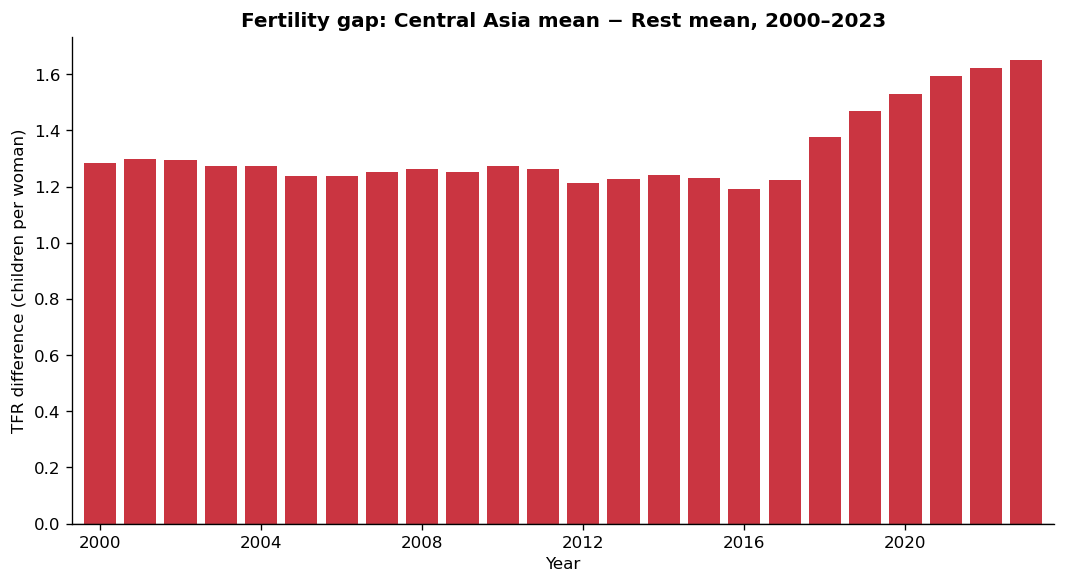
\includegraphics[width=0.88\textwidth]{figures/fig4_gap}
  \caption{Difference between Central Asian and other post-Soviet mean total fertility rates, 2000--2023.}
  \label{fig:gap}
\end{figure}

It is worth being precise about where that widening came from, because the intuitive reading is misleading. Central Asia did rise after 2016, by 0.13 children per woman. But the comparison bloc fell by 0.33 over the same years. Of the total widening of 0.46, roughly seventy per cent is the rest of the post-Soviet space declining and only thirty per cent is Central Asia climbing. The divergence is therefore as much a story about Ukraine, Lithuania, Latvia and Belarus as it is about Uzbekistan, and any account that treats it purely as a Central Asian phenomenon is describing less than a third of the movement.

Disaggregating the comparison bloc confirms that the decline is broad rather than driven by one sub-region. Between 2016 and 2023 the Baltic mean fell from 1.68 to 1.30, the Eastern European mean from 1.70 to 1.34, and the Caucasus mean from 1.96 to 1.73. All three moved in the same direction over the same years. The Caucasus remains the intermediate case throughout, sitting consistently above the Baltic and Eastern European groups and well below Central Asia, which is what one would expect of a region that shares some of Central Asia's cultural and nuptiality characteristics without sharing all of them. The sub-group series are reported in Appendix~\ref{app:subgroups}.

\subsection{Convergence and divergence}
\label{sec:convergence}

If the post-Soviet states had been converging on a common fertility regime, dispersion across them should have fallen. The standard way to test this is $\sigma$-convergence: the coefficient of variation of fertility computed across countries within each year.

Taken over the full window, the answer looks like nothing happened. The coefficient of variation was 0.398 in 2000 and 0.428 in 2023, and a linear trend through the whole series gives a slope of $-0.0007$ per year with a p-value of 0.758. Read on its own, that says the fourteen countries were no more alike at the end than at the beginning.

That reading is wrong in an instructive way, because the flat trend is the average of two things moving in opposite directions. The left panel of Figure~\ref{fig:sigma} shows the pooled series falling steadily from 2000 to a minimum of 0.292 in 2016, then rising sharply to 0.428 by 2023. Fitted separately, the two phases give slopes of $-0.0072$ per year over 2000--2016 ($p < 0.001$) and $+0.0195$ per year afterwards. The second figure carries no p-value: seven annual observations are not enough for reliable inference on a serially correlated series, so only the sign and the visible pattern are claimed. The post-2016 window is short, but the direction is unambiguous and, as Section~\ref{sec:desc-robust} shows, it survives every check applied to it.

\begin{figure}[htbp]
  \centering
  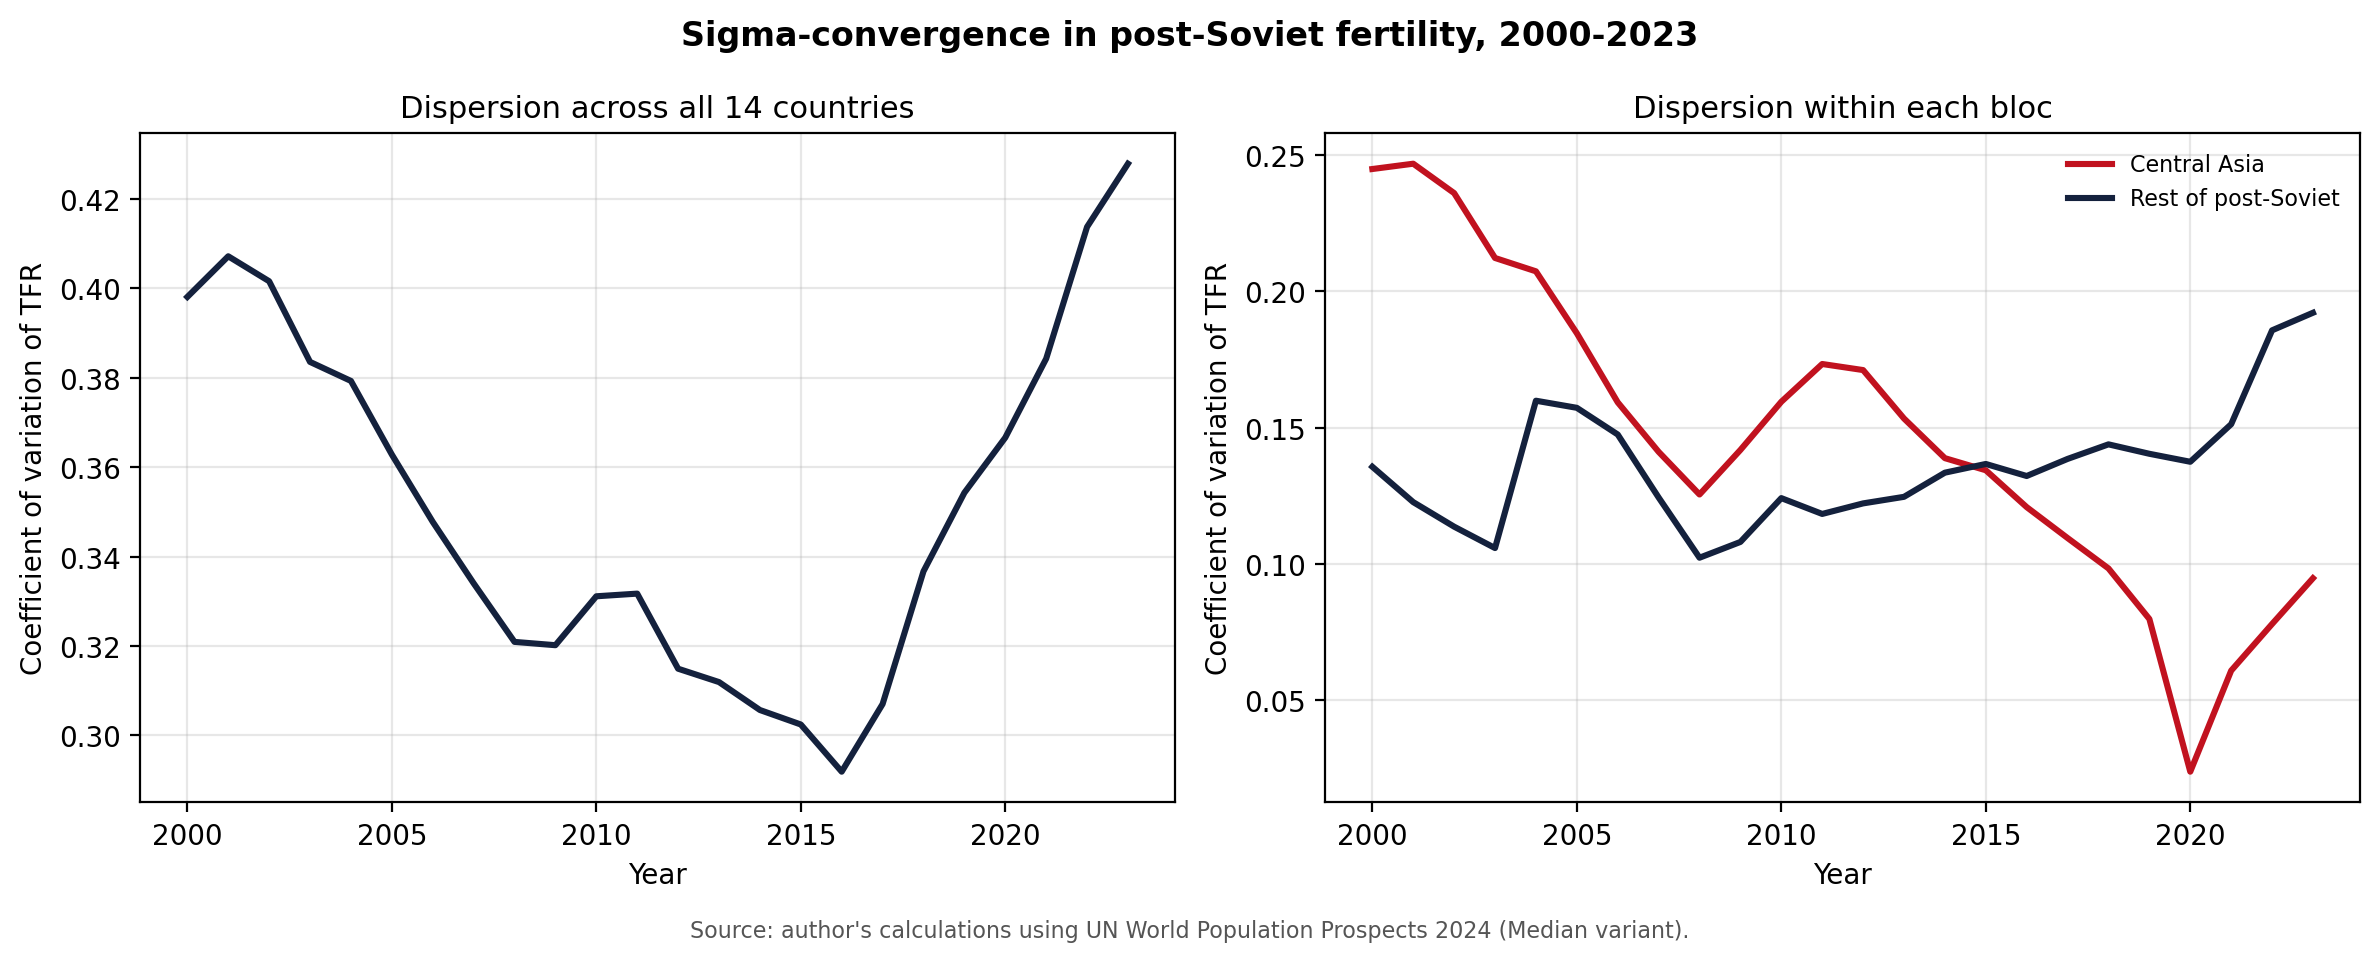
\includegraphics[width=\textwidth]{figures/fig5_sigma_convergence}
  \caption{$\sigma$-convergence in post-Soviet fertility. Left: dispersion across all fourteen countries. Right: dispersion within each bloc.}
  \label{fig:sigma}
\end{figure}

The second decomposition matters more. The right panel splits dispersion by bloc, and the two lines run in opposite directions. Within Central Asia, dispersion falls steeply and significantly, at $-0.0075$ per year ($p < 0.001$). Within the rest of the post-Soviet space it rises, at $+0.0016$ per year ($p = 0.025$). The four Central Asian countries have been growing more alike while the other ten have been growing less alike, and the pooled series in the left panel is simply these two movements cancelling.

Because the coefficient of variation is a ratio, a fall in it can reflect a rising mean rather than genuine compression. Here it does not. Central Asia's standard deviation fell from 0.653 in 2000 to 0.293 in 2023, and its interquartile range from 0.488 to 0.220; the comparison bloc's standard deviation rose from 0.187 to 0.278 and its interquartile range from 0.238 to 0.463. Both movements appear in absolute dispersion, not only in the scale-free measure, so neither is a denominator artefact. Note also that pooled absolute dispersion increased over the period (standard deviation 0.696 to 0.820) even though the pooled coefficient of variation barely moved, which is a further reminder that the ratio alone would have been misleading.

Two of these trends depend on particular countries and should be reported as such. Central Asia's internal convergence loses statistical significance when Tajikistan is dropped ($p = 0.132$), which makes sense: Tajikistan started highest and declined while the others rose, so it is doing much of the work of compressing the bloc. The comparison bloc's divergence loses significance when either Georgia ($p = 0.485$) or Ukraine ($p = 0.632$) is removed. These are country-sensitive patterns rather than group-wide regularities, and the leave-one-out results are given in full in Appendix~\ref{app:loo-convergence}.

The complementary test asks whether initially higher-fertility countries fell faster --- $\beta$-convergence. They did not. Estimating equation~\eqref{eq:beta} on the fourteen countries gives $\beta = +0.0013$ (HC3 standard error 0.0116, $p = 0.911$), with a confidence interval from $-0.024$ to $+0.027$ and an $R^2$ of 0.004. The point estimate is positive, meaning if anything that countries starting higher grew faster still, but it is indistinguishable from zero and the specification explains essentially none of the variation. Adding the Central Asia indicator raises $R^2$ to 0.270 without either coefficient reaching conventional significance (initial level $-0.020$, $p = 0.467$; Central Asia $+0.018$, $p = 0.368$). With fourteen observations this is a weak test, and the caution about regression to the mean noted in Section~\ref{sec:descriptive-methods} applies \parencite{quah1993}. What can be said is that the data offer no evidence of catch-up in either direction.

\subsection{The turning point after 2016}
\label{sec:turning-point}

Several of the results above locate a break at the same place. Pooled dispersion reaches its minimum in 2016 and rises thereafter. The bloc difference is at its narrowest in the same year. The comparison bloc's mean peaks in 2016 and declines from then on. Ten of the fourteen countries record their highest fertility in 2015 or later, which means the peak and the reversal are close together almost everywhere.

The single largest movement in the panel belongs to Uzbekistan, whose rate went from 2.57 in 2017 to 3.50 in 2023 --- an increase of 0.93 children per woman in six years, and the reason Uzbekistan holds the highest value in the sample by 2023 despite having been the second lowest of the four Central Asian countries in 2000. Kazakhstan's trajectory over the full window is almost as remarkable in a different way: from 1.90 in 2000, a level then comparable to Azerbaijan's, to 3.01 in 2023, a gain of 1.11 children per woman. These are not marginal adjustments to an existing regime.

At the other end, the declines after 2017 are broad and, in several countries, steep: Lithuania $-0.43$, Latvia $-0.36$, Belarus $-0.34$, Georgia $-0.33$, Ukraine $-0.32$, Azerbaijan $-0.29$. Nine of the ten countries outside Central Asia declined over these six years, Armenia being the single exception. Ukraine's fall is partly attributable to the full-scale invasion in 2022 and the displacement that followed, but the decline was underway before it: Ukraine had already dropped from 1.30 in 2017 to 1.15 by 2021.

It should be said clearly what this section does and does not establish. It documents a change in period fertility rates that is simultaneous across a large part of the sample and coincides with a visible break in dispersion. It does not identify what produced the break, and period rates cannot separate a genuine change in family size from a change in the timing of births \parencite{bongaarts1998}. That ten of fourteen countries peaked within a few years of each other is consistent with a common shift in the pace of postponement as much as with a common change in intended family size, and this analysis cannot tell the two apart.

\subsection{Are the descriptive results robust?}
\label{sec:desc-robust}

Two of the findings above --- the post-2016 rise in dispersion and the $\beta$ estimate --- depend on the end of the series, which is exactly where the World Population Prospects data are weakest, since eleven of the fourteen 2023 values are projections. Both are therefore recomputed on the two balanced sub-samples described in Section~\ref{sec:proj-check}.

The post-2016 dispersion slope is positive in all three samples: $+0.0195$ in the full sample, $+0.0237$ using all fourteen countries over 2000--2019 with no projected values anywhere, and $+0.0261$ using the ten countries with a non-projected observation in every year from 2017 to 2022. Rather than casting doubt on the divergence result, the exercise strengthens it: the finding is not an artefact of projected endpoints, and it is not an artefact of a shrinking, low-fertility-biased country set. The $\beta$ estimate is less stable --- $+0.0013$, $-0.0085$ and $+0.0052$ across the three samples --- but nothing rests on its sign, and all three are consistent with the conclusion that there is no detectable catch-up. Full results appear in Appendix~\ref{app:projection-check}.

\subsection{Summary}
\label{sec:trends-summary}

Fertility in the post-Soviet space did not converge between 2000 and 2023. The four Central Asian countries remained above the other ten in every single year, with no crossing at any point, and the difference between the two groups ended the period wider than it began. Underneath a flat pooled dispersion series, Central Asia converged internally while the rest of the region pulled apart. There is no evidence of catch-up: initially higher-fertility countries did not decline faster. And around 2016 the pattern changed, with a broad-based decline outside Central Asia accounting for roughly seventy per cent of a widening difference that reached 1.65 children per woman by 2023.

The remainder of the thesis takes that difference as its object. Chapter~\ref{sec:premium} asks how much of it moves together with observable economic conditions, and how much does not.

%  Requires: \input or \include of tables/tab_country_tfr.tex, and the
%  four PNG figures in figures/.
% =====================================================================

\section{Fertility Trends in the Post-Soviet Space, 2000--2023}
\label{sec:trends}

\subsection{Levels and trajectories}
\label{sec:levels}

In 2000 the fourteen countries in this study ranged from 1.11 children per woman in Ukraine to 3.49 in Tajikistan. Twenty-three years later the range had not narrowed. Ukraine had fallen to 0.98, one of the lowest national fertility rates ever recorded anywhere, while Uzbekistan had risen to 3.50. The endpoints are almost identical to where they started; what changed is which countries occupy them and how they got there.

\begin{table}[htbp]
\centering
\caption{Total fertility rate at selected dates, 2000--2023}
\label{tab:country-tfr}
\small
\begin{tabular}{lrrrrrr}
\toprule
 & 2000 & 2010 & 2017 & 2023 & $\Delta$ 2000--23 & $\Delta$ 2017--23 \\
\midrule
\multicolumn{7}{l}{\textit{Central Asia}} \\
\quad Kazakhstan & 1.90 & 2.61 & 2.75 & 3.01 & +1.11 & +0.27 \\
\quad Kyrgyzstan & 2.58 & 3.10 & 3.04 & 2.80 & +0.22 & -0.24 \\
\quad Tajikistan & 3.49 & 3.46 & 3.29 & 3.07 & -0.42 & -0.22 \\
\quad Uzbekistan & 2.70 & 2.44 & 2.57 & 3.50 & +0.80 & +0.93 \\
\addlinespace
\quad \textit{Bloc mean} & 2.67 & 2.90 & 2.91 & 3.10 & +0.43 & +0.18 \\
\addlinespace
\multicolumn{7}{l}{\textit{Rest of post-Soviet space}} \\
\quad Armenia & 1.47 & 1.59 & 1.56 & 1.71 & +0.24 & +0.15 \\
\quad Azerbaijan & 1.70 & 1.92 & 1.96 & 1.67 & -0.03 & -0.29 \\
\quad Belarus & 1.27 & 1.48 & 1.55 & 1.21 & -0.06 & -0.34 \\
\quad Estonia & 1.35 & 1.72 & 1.60 & 1.35 & +0.00 & -0.25 \\
\quad Georgia & 1.61 & 1.97 & 2.14 & 1.81 & +0.20 & -0.33 \\
\quad Latvia & 1.24 & 1.37 & 1.70 & 1.34 & +0.09 & -0.36 \\
\quad Lithuania & 1.38 & 1.50 & 1.63 & 1.20 & -0.18 & -0.43 \\
\quad Moldova & 1.50 & 1.70 & 1.81 & 1.73 & +0.23 & -0.08 \\
\quad Russia & 1.19 & 1.59 & 1.63 & 1.45 & +0.26 & -0.18 \\
\quad Ukraine & 1.11 & 1.44 & 1.30 & 0.98 & -0.13 & -0.32 \\
\addlinespace
\quad \textit{Bloc mean} & 1.38 & 1.63 & 1.69 & 1.44 & +0.06 & -0.24 \\
\addlinespace
\midrule
\multicolumn{7}{l}{Difference in bloc means} \\
\quad Central Asia $-$ rest & 1.28 & 1.27 & 1.23 & 1.65 & & \\
\bottomrule
\end{tabular}

\begin{minipage}{\textwidth}\footnotesize
\vspace{4pt}
\emph{Source:} UN World Population Prospects 2024, median variant; author's calculations.
\emph{Note:} Bloc means and differences are computed from unrounded country values,
so they need not equal the difference of the rounded figures shown. Eleven of the
fourteen 2023 values are WPP projections rather than retrospective interpolated
estimates; only Latvia, Lithuania and Russia are interpolated in 2023.
\end{minipage}
\end{table}

Table~\ref{tab:country-tfr} sets out the individual trajectories, and Figure~\ref{fig:all-countries} shows all fourteen together. Two things stand out immediately. The first is the separation. In every single year of the panel, the lowest-fertility Central Asian country lies above the highest-fertility country outside Central Asia. There is not one crossing in twenty-four years, and the narrowest the two groups ever come is 0.195 children per woman, in 2012.

\begin{figure}[htbp]
  \centering
  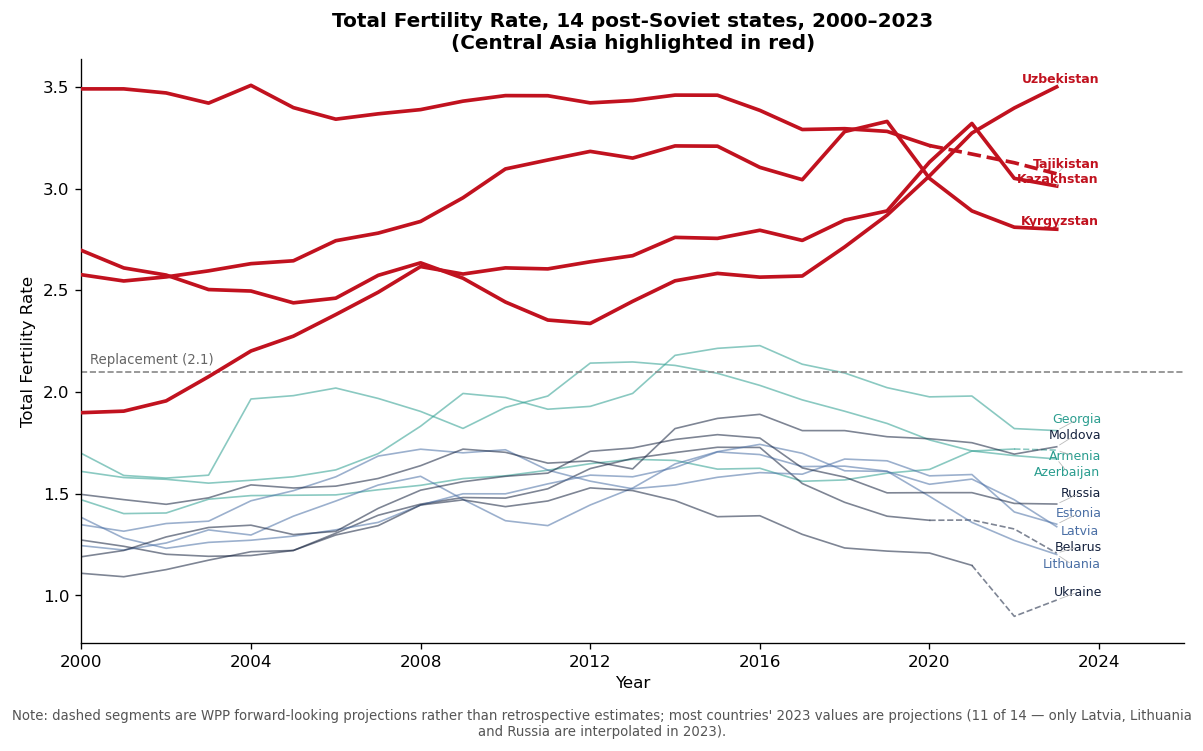
\includegraphics[width=\textwidth]{figures/fig1_all_countries}
  \caption{Total fertility rate, fourteen post-Soviet states, 2000--2023. Central Asian countries in red. Dashed segments are WPP forward-looking projections rather than retrospective estimates.}
  \label{fig:all-countries}
\end{figure}

The second is that the separation does not come from a shared decline at different speeds. Most of the sample rose for the first fifteen years or so. Ten of the fourteen countries recorded their highest fertility of the period in 2015 or later, and only Tajikistan among the Central Asian states peaked early, in 2004. Russia's rate climbed from 1.19 to a high of 1.79 in 2015 before falling back; Latvia went from 1.24 to 1.74 in 2016; Georgia reached 2.23 in 2016, briefly above replacement. This broad recovery from the post-Soviet trough is well documented for the European successor states \parencite{billingsley2010,grigoras2019} and for Central Asia \parencite{spoorenberg2015}. What has not been documented, because the comparative literature ends before it, is what happened after that.

By 2023 ten of the fourteen countries were below the replacement level of 2.1, and the four that were not are the four Central Asian states. Three of the ten European and Caucasian countries had fallen below 1.25.

\subsection{The difference between the blocs}
\label{sec:gap}

Figure~\ref{fig:bloc-means} tracks the two bloc means with the country range around each. The Central Asian mean rose from 2.67 in 2000 to 3.09 in 2023, an increase of 0.43 children per woman. The rest of the post-Soviet space rose too, from 1.38 to a peak of 1.77 in 2016, and then gave nearly all of it back, ending at 1.44.

\begin{figure}[htbp]
  \centering
  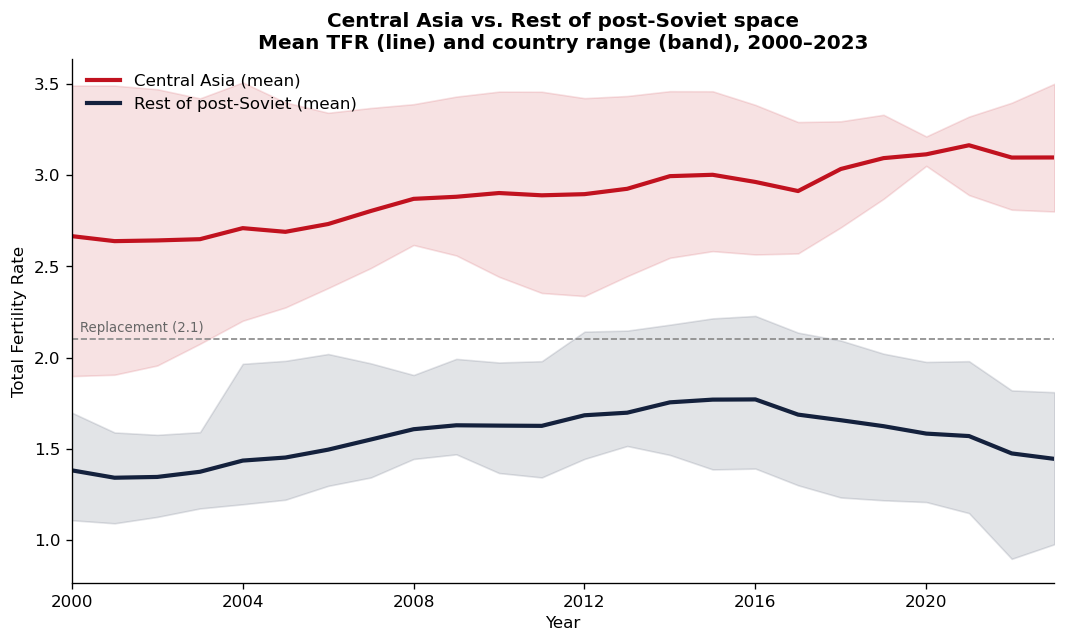
\includegraphics[width=0.92\textwidth]{figures/fig2_bloc_means}
  \caption{Mean total fertility rate by bloc, with the country range shown as a shaded band, 2000--2023.}
  \label{fig:bloc-means}
\end{figure}

The difference between the two means is the central descriptive object of this thesis, and its behaviour over time is more interesting than its average size. Figure~\ref{fig:gap} plots it year by year. From 2000 to 2016 it is remarkably flat, moving within a narrow corridor between 1.19 and 1.30 and drifting very slightly downward. Then it changes character: 1.19 in 2016, 1.38 in 2018, 1.53 in 2020, 1.65 in 2023. Over seven years it widened by 0.46 children per woman, having barely moved in the previous sixteen.

\begin{figure}[htbp]
  \centering
  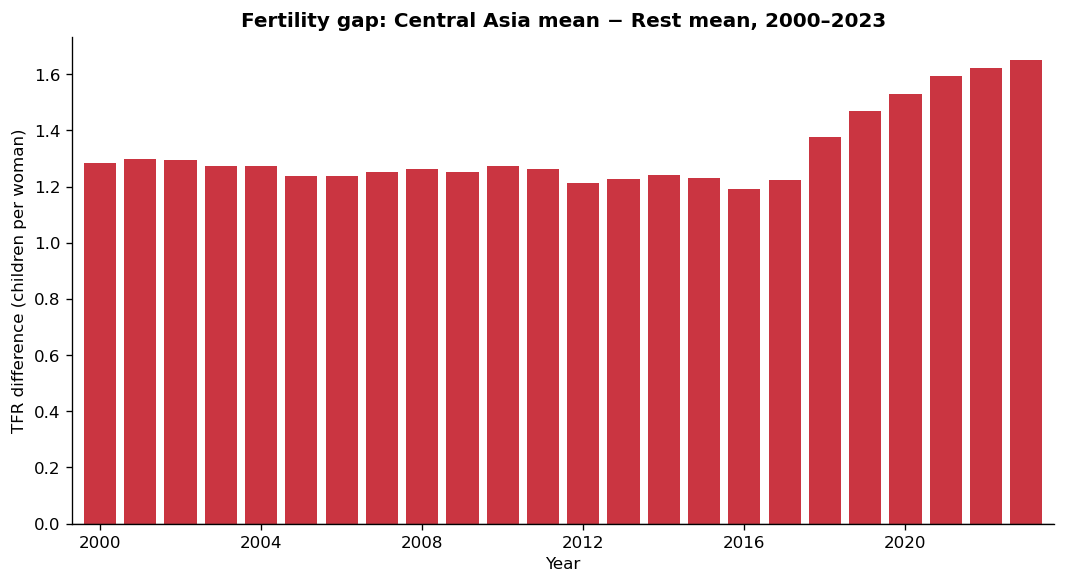
\includegraphics[width=0.88\textwidth]{figures/fig4_gap}
  \caption{Difference between Central Asian and other post-Soviet mean total fertility rates, 2000--2023.}
  \label{fig:gap}
\end{figure}

It is worth being precise about where that widening came from, because the intuitive reading is misleading. Central Asia did rise after 2016, by 0.13 children per woman. But the comparison bloc fell by 0.33 over the same years. Of the total widening of 0.46, roughly seventy per cent is the rest of the post-Soviet space declining and only thirty per cent is Central Asia climbing. The divergence is therefore as much a story about Ukraine, Lithuania, Latvia and Belarus as it is about Uzbekistan, and any account that treats it purely as a Central Asian phenomenon is describing less than a third of the movement.

Disaggregating the comparison bloc confirms that the decline is broad rather than driven by one sub-region. Between 2016 and 2023 the Baltic mean fell from 1.68 to 1.30, the Eastern European mean from 1.70 to 1.34, and the Caucasus mean from 1.96 to 1.73. All three moved in the same direction over the same years. The Caucasus remains the intermediate case throughout, sitting consistently above the Baltic and Eastern European groups and well below Central Asia, which is what one would expect of a region that shares some of Central Asia's cultural and nuptiality characteristics without sharing all of them. The sub-group series are reported in Appendix~\ref{app:subgroups}.

\subsection{Convergence and divergence}
\label{sec:convergence}

If the post-Soviet states had been converging on a common fertility regime, dispersion across them should have fallen. The standard way to test this is $\sigma$-convergence: the coefficient of variation of fertility computed across countries within each year.

Taken over the full window, the answer looks like nothing happened. The coefficient of variation was 0.398 in 2000 and 0.428 in 2023, and a linear trend through the whole series gives a slope of $-0.0007$ per year with a p-value of 0.758. Read on its own, that says the fourteen countries were no more alike at the end than at the beginning.

That reading is wrong in an instructive way, because the flat trend is the average of two things moving in opposite directions. The left panel of Figure~\ref{fig:sigma} shows the pooled series falling steadily from 2000 to a minimum of 0.292 in 2016, then rising sharply to 0.428 by 2023. Fitted separately, the two phases give slopes of $-0.0072$ per year over 2000--2016 ($p < 0.001$) and $+0.0195$ per year afterwards. The second figure carries no p-value: seven annual observations are not enough for reliable inference on a serially correlated series, so only the sign and the visible pattern are claimed. The post-2016 window is short, but the direction is unambiguous and, as Section~\ref{sec:desc-robust} shows, it survives every check applied to it.

\begin{figure}[htbp]
  \centering
  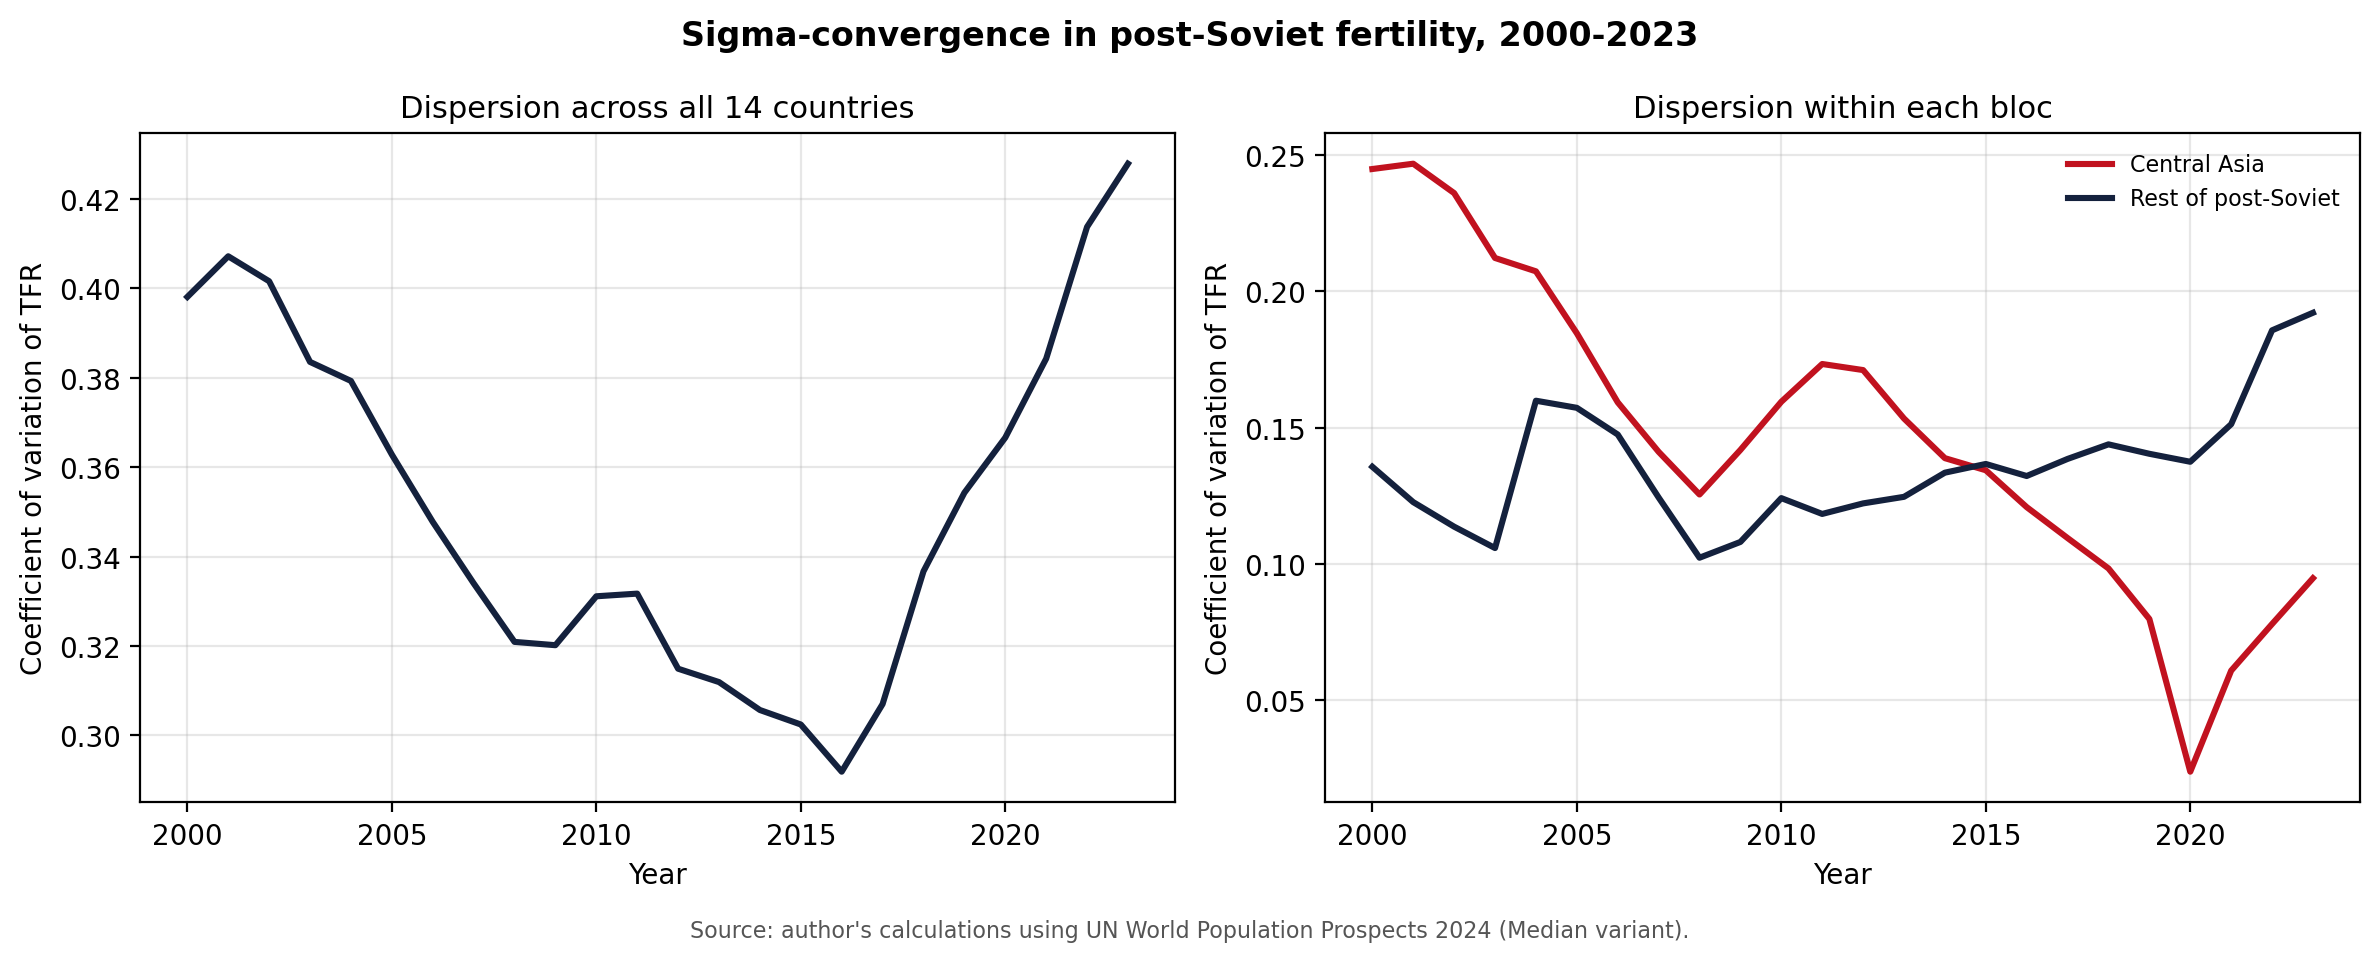
\includegraphics[width=\textwidth]{figures/fig5_sigma_convergence}
  \caption{$\sigma$-convergence in post-Soviet fertility. Left: dispersion across all fourteen countries. Right: dispersion within each bloc.}
  \label{fig:sigma}
\end{figure}

The second decomposition matters more. The right panel splits dispersion by bloc, and the two lines run in opposite directions. Within Central Asia, dispersion falls steeply and significantly, at $-0.0075$ per year ($p < 0.001$). Within the rest of the post-Soviet space it rises, at $+0.0016$ per year ($p = 0.025$). The four Central Asian countries have been growing more alike while the other ten have been growing less alike, and the pooled series in the left panel is simply these two movements cancelling.

Because the coefficient of variation is a ratio, a fall in it can reflect a rising mean rather than genuine compression. Here it does not. Central Asia's standard deviation fell from 0.653 in 2000 to 0.293 in 2023, and its interquartile range from 0.488 to 0.220; the comparison bloc's standard deviation rose from 0.187 to 0.278 and its interquartile range from 0.238 to 0.463. Both movements appear in absolute dispersion, not only in the scale-free measure, so neither is a denominator artefact. Note also that pooled absolute dispersion increased over the period (standard deviation 0.696 to 0.820) even though the pooled coefficient of variation barely moved, which is a further reminder that the ratio alone would have been misleading.

Two of these trends depend on particular countries and should be reported as such. Central Asia's internal convergence loses statistical significance when Tajikistan is dropped ($p = 0.132$), which makes sense: Tajikistan started highest and declined while the others rose, so it is doing much of the work of compressing the bloc. The comparison bloc's divergence loses significance when either Georgia ($p = 0.485$) or Ukraine ($p = 0.632$) is removed. These are country-sensitive patterns rather than group-wide regularities, and the leave-one-out results are given in full in Appendix~\ref{app:loo-convergence}.

The complementary test asks whether initially higher-fertility countries fell faster --- $\beta$-convergence. They did not. Estimating equation~\eqref{eq:beta} on the fourteen countries gives $\beta = +0.0013$ (HC3 standard error 0.0116, $p = 0.911$), with a confidence interval from $-0.024$ to $+0.027$ and an $R^2$ of 0.004. The point estimate is positive, meaning if anything that countries starting higher grew faster still, but it is indistinguishable from zero and the specification explains essentially none of the variation. Adding the Central Asia indicator raises $R^2$ to 0.270 without either coefficient reaching conventional significance (initial level $-0.020$, $p = 0.467$; Central Asia $+0.018$, $p = 0.368$). With fourteen observations this is a weak test, and the caution about regression to the mean noted in Section~\ref{sec:descriptive-methods} applies \parencite{quah1993}. What can be said is that the data offer no evidence of catch-up in either direction.

\subsection{The turning point after 2016}
\label{sec:turning-point}

Several of the results above locate a break at the same place. Pooled dispersion reaches its minimum in 2016 and rises thereafter. The bloc difference is at its narrowest in the same year. The comparison bloc's mean peaks in 2016 and declines from then on. Ten of the fourteen countries record their highest fertility in 2015 or later, which means the peak and the reversal are close together almost everywhere.

The single largest movement in the panel belongs to Uzbekistan, whose rate went from 2.57 in 2017 to 3.50 in 2023 --- an increase of 0.93 children per woman in six years, and the reason Uzbekistan holds the highest value in the sample by 2023 despite having been the second lowest of the four Central Asian countries in 2000. Kazakhstan's trajectory over the full window is almost as remarkable in a different way: from 1.90 in 2000, a level then comparable to Azerbaijan's, to 3.01 in 2023, a gain of 1.11 children per woman. These are not marginal adjustments to an existing regime.

At the other end, the declines after 2017 are broad and, in several countries, steep: Lithuania $-0.43$, Latvia $-0.36$, Belarus $-0.34$, Georgia $-0.33$, Ukraine $-0.32$, Azerbaijan $-0.29$. Nine of the ten countries outside Central Asia declined over these six years, Armenia being the single exception. Ukraine's fall is partly attributable to the full-scale invasion in 2022 and the displacement that followed, but the decline was underway before it: Ukraine had already dropped from 1.30 in 2017 to 1.15 by 2021.

It should be said clearly what this section does and does not establish. It documents a change in period fertility rates that is simultaneous across a large part of the sample and coincides with a visible break in dispersion. It does not identify what produced the break, and period rates cannot separate a genuine change in family size from a change in the timing of births \parencite{bongaarts1998}. That ten of fourteen countries peaked within a few years of each other is consistent with a common shift in the pace of postponement as much as with a common change in intended family size, and this analysis cannot tell the two apart.

\subsection{Are the descriptive results robust?}
\label{sec:desc-robust}

Two of the findings above --- the post-2016 rise in dispersion and the $\beta$ estimate --- depend on the end of the series, which is exactly where the World Population Prospects data are weakest, since eleven of the fourteen 2023 values are projections. Both are therefore recomputed on the two balanced sub-samples described in Section~\ref{sec:proj-check}.

The post-2016 dispersion slope is positive in all three samples: $+0.0195$ in the full sample, $+0.0237$ using all fourteen countries over 2000--2019 with no projected values anywhere, and $+0.0261$ using the ten countries with a non-projected observation in every year from 2017 to 2022. Rather than casting doubt on the divergence result, the exercise strengthens it: the finding is not an artefact of projected endpoints, and it is not an artefact of a shrinking, low-fertility-biased country set. The $\beta$ estimate is less stable --- $+0.0013$, $-0.0085$ and $+0.0052$ across the three samples --- but nothing rests on its sign, and all three are consistent with the conclusion that there is no detectable catch-up. Full results appear in Appendix~\ref{app:projection-check}.

\subsection{Summary}
\label{sec:trends-summary}

Fertility in the post-Soviet space did not converge between 2000 and 2023. The four Central Asian countries remained above the other ten in every single year, with no crossing at any point, and the difference between the two groups ended the period wider than it began. Underneath a flat pooled dispersion series, Central Asia converged internally while the rest of the region pulled apart. There is no evidence of catch-up: initially higher-fertility countries did not decline faster. And around 2016 the pattern changed, with a broad-based decline outside Central Asia accounting for roughly seventy per cent of a widening difference that reached 1.65 children per woman by 2023.

The remainder of the thesis takes that difference as its object. Chapter~\ref{sec:premium} asks how much of it moves together with observable economic conditions, and how much does not.

%  Requires: \input or \include of tables/tab_country_tfr.tex, and the
%  four PNG figures in figures/.
% =====================================================================

\section{Fertility Trends in the Post-Soviet Space, 2000--2023}
\label{sec:trends}

\subsection{Levels and trajectories}
\label{sec:levels}

In 2000 the fourteen countries in this study ranged from 1.11 children per woman in Ukraine to 3.49 in Tajikistan. Twenty-three years later the range had not narrowed. Ukraine had fallen to 0.98, one of the lowest national fertility rates ever recorded anywhere, while Uzbekistan had risen to 3.50. The endpoints are almost identical to where they started; what changed is which countries occupy them and how they got there.

\begin{table}[htbp]
\centering
\caption{Total fertility rate at selected dates, 2000--2023}
\label{tab:country-tfr}
\small
\begin{tabular}{lrrrrrr}
\toprule
 & 2000 & 2010 & 2017 & 2023 & $\Delta$ 2000--23 & $\Delta$ 2017--23 \\
\midrule
\multicolumn{7}{l}{\textit{Central Asia}} \\
\quad Kazakhstan & 1.90 & 2.61 & 2.75 & 3.01 & +1.11 & +0.27 \\
\quad Kyrgyzstan & 2.58 & 3.10 & 3.04 & 2.80 & +0.22 & -0.24 \\
\quad Tajikistan & 3.49 & 3.46 & 3.29 & 3.07 & -0.42 & -0.22 \\
\quad Uzbekistan & 2.70 & 2.44 & 2.57 & 3.50 & +0.80 & +0.93 \\
\addlinespace
\quad \textit{Bloc mean} & 2.67 & 2.90 & 2.91 & 3.10 & +0.43 & +0.18 \\
\addlinespace
\multicolumn{7}{l}{\textit{Rest of post-Soviet space}} \\
\quad Armenia & 1.47 & 1.59 & 1.56 & 1.71 & +0.24 & +0.15 \\
\quad Azerbaijan & 1.70 & 1.92 & 1.96 & 1.67 & -0.03 & -0.29 \\
\quad Belarus & 1.27 & 1.48 & 1.55 & 1.21 & -0.06 & -0.34 \\
\quad Estonia & 1.35 & 1.72 & 1.60 & 1.35 & +0.00 & -0.25 \\
\quad Georgia & 1.61 & 1.97 & 2.14 & 1.81 & +0.20 & -0.33 \\
\quad Latvia & 1.24 & 1.37 & 1.70 & 1.34 & +0.09 & -0.36 \\
\quad Lithuania & 1.38 & 1.50 & 1.63 & 1.20 & -0.18 & -0.43 \\
\quad Moldova & 1.50 & 1.70 & 1.81 & 1.73 & +0.23 & -0.08 \\
\quad Russia & 1.19 & 1.59 & 1.63 & 1.45 & +0.26 & -0.18 \\
\quad Ukraine & 1.11 & 1.44 & 1.30 & 0.98 & -0.13 & -0.32 \\
\addlinespace
\quad \textit{Bloc mean} & 1.38 & 1.63 & 1.69 & 1.44 & +0.06 & -0.24 \\
\addlinespace
\midrule
\multicolumn{7}{l}{Difference in bloc means} \\
\quad Central Asia $-$ rest & 1.28 & 1.27 & 1.23 & 1.65 & & \\
\bottomrule
\end{tabular}

\begin{minipage}{\textwidth}\footnotesize
\vspace{4pt}
\emph{Source:} UN World Population Prospects 2024, median variant; author's calculations.
\emph{Note:} Bloc means and differences are computed from unrounded country values,
so they need not equal the difference of the rounded figures shown. Eleven of the
fourteen 2023 values are WPP projections rather than retrospective interpolated
estimates; only Latvia, Lithuania and Russia are interpolated in 2023.
\end{minipage}
\end{table}

Table~\ref{tab:country-tfr} sets out the individual trajectories, and Figure~\ref{fig:all-countries} shows all fourteen together. Two things stand out immediately. The first is the separation. In every single year of the panel, the lowest-fertility Central Asian country lies above the highest-fertility country outside Central Asia. There is not one crossing in twenty-four years, and the narrowest the two groups ever come is 0.195 children per woman, in 2012.

\begin{figure}[htbp]
  \centering
  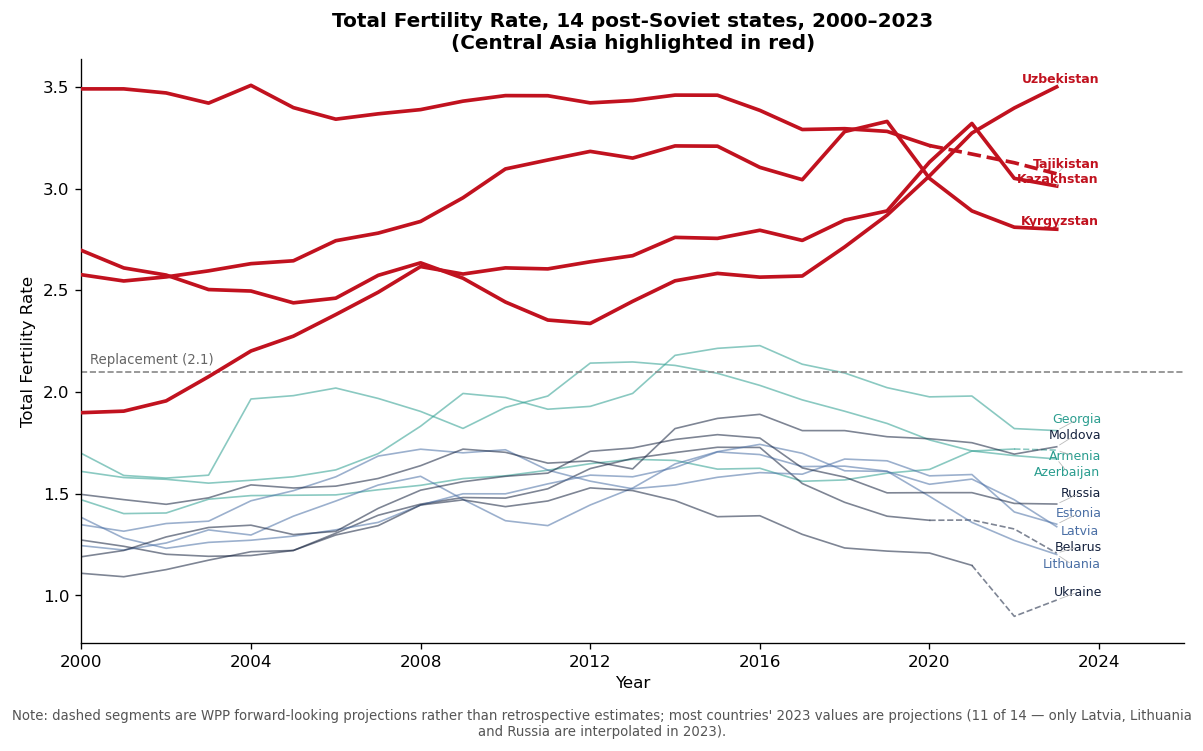
\includegraphics[width=\textwidth]{figures/fig1_all_countries}
  \caption{Total fertility rate, fourteen post-Soviet states, 2000--2023. Central Asian countries in red. Dashed segments are WPP forward-looking projections rather than retrospective estimates.}
  \label{fig:all-countries}
\end{figure}

The second is that the separation does not come from a shared decline at different speeds. Most of the sample rose for the first fifteen years or so. Ten of the fourteen countries recorded their highest fertility of the period in 2015 or later, and only Tajikistan among the Central Asian states peaked early, in 2004. Russia's rate climbed from 1.19 to a high of 1.79 in 2015 before falling back; Latvia went from 1.24 to 1.74 in 2016; Georgia reached 2.23 in 2016, briefly above replacement. This broad recovery from the post-Soviet trough is well documented for the European successor states \parencite{billingsley2010,grigoras2019} and for Central Asia \parencite{spoorenberg2015}. What has not been documented, because the comparative literature ends before it, is what happened after that.

By 2023 ten of the fourteen countries were below the replacement level of 2.1, and the four that were not are the four Central Asian states. Three of the ten European and Caucasian countries had fallen below 1.25.

\subsection{The difference between the blocs}
\label{sec:gap}

Figure~\ref{fig:bloc-means} tracks the two bloc means with the country range around each. The Central Asian mean rose from 2.67 in 2000 to 3.09 in 2023, an increase of 0.43 children per woman. The rest of the post-Soviet space rose too, from 1.38 to a peak of 1.77 in 2016, and then gave nearly all of it back, ending at 1.44.

\begin{figure}[htbp]
  \centering
  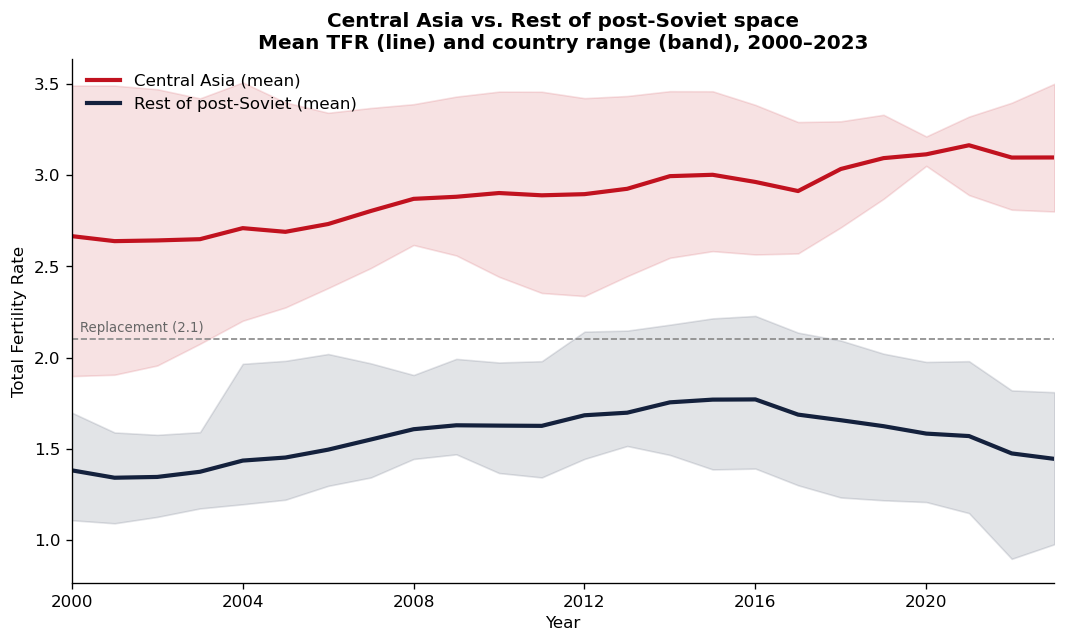
\includegraphics[width=0.92\textwidth]{figures/fig2_bloc_means}
  \caption{Mean total fertility rate by bloc, with the country range shown as a shaded band, 2000--2023.}
  \label{fig:bloc-means}
\end{figure}

The difference between the two means is the central descriptive object of this thesis, and its behaviour over time is more interesting than its average size. Figure~\ref{fig:gap} plots it year by year. From 2000 to 2016 it is remarkably flat, moving within a narrow corridor between 1.19 and 1.30 and drifting very slightly downward. Then it changes character: 1.19 in 2016, 1.38 in 2018, 1.53 in 2020, 1.65 in 2023. Over seven years it widened by 0.46 children per woman, having barely moved in the previous sixteen.

\begin{figure}[htbp]
  \centering
  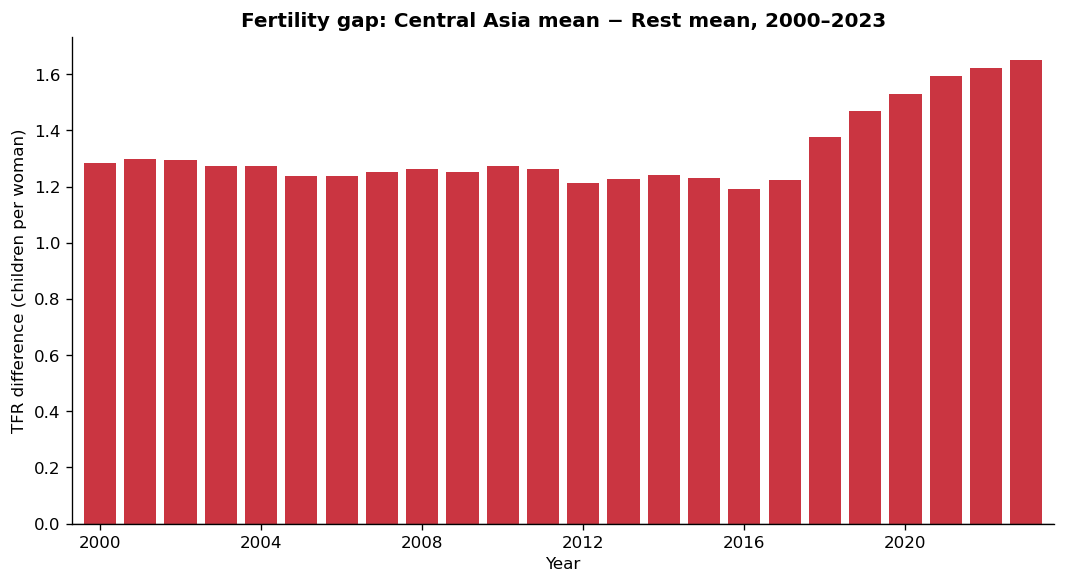
\includegraphics[width=0.88\textwidth]{figures/fig4_gap}
  \caption{Difference between Central Asian and other post-Soviet mean total fertility rates, 2000--2023.}
  \label{fig:gap}
\end{figure}

It is worth being precise about where that widening came from, because the intuitive reading is misleading. Central Asia did rise after 2016, by 0.13 children per woman. But the comparison bloc fell by 0.33 over the same years. Of the total widening of 0.46, roughly seventy per cent is the rest of the post-Soviet space declining and only thirty per cent is Central Asia climbing. The divergence is therefore as much a story about Ukraine, Lithuania, Latvia and Belarus as it is about Uzbekistan, and any account that treats it purely as a Central Asian phenomenon is describing less than a third of the movement.

Disaggregating the comparison bloc confirms that the decline is broad rather than driven by one sub-region. Between 2016 and 2023 the Baltic mean fell from 1.68 to 1.30, the Eastern European mean from 1.70 to 1.34, and the Caucasus mean from 1.96 to 1.73. All three moved in the same direction over the same years. The Caucasus remains the intermediate case throughout, sitting consistently above the Baltic and Eastern European groups and well below Central Asia, which is what one would expect of a region that shares some of Central Asia's cultural and nuptiality characteristics without sharing all of them. The sub-group series are reported in Appendix~\ref{app:subgroups}.

\subsection{Convergence and divergence}
\label{sec:convergence}

If the post-Soviet states had been converging on a common fertility regime, dispersion across them should have fallen. The standard way to test this is $\sigma$-convergence: the coefficient of variation of fertility computed across countries within each year.

Taken over the full window, the answer looks like nothing happened. The coefficient of variation was 0.398 in 2000 and 0.428 in 2023, and a linear trend through the whole series gives a slope of $-0.0007$ per year with a p-value of 0.758. Read on its own, that says the fourteen countries were no more alike at the end than at the beginning.

That reading is wrong in an instructive way, because the flat trend is the average of two things moving in opposite directions. The left panel of Figure~\ref{fig:sigma} shows the pooled series falling steadily from 2000 to a minimum of 0.292 in 2016, then rising sharply to 0.428 by 2023. Fitted separately, the two phases give slopes of $-0.0072$ per year over 2000--2016 ($p < 0.001$) and $+0.0195$ per year afterwards. The second figure carries no p-value: seven annual observations are not enough for reliable inference on a serially correlated series, so only the sign and the visible pattern are claimed. The post-2016 window is short, but the direction is unambiguous and, as Section~\ref{sec:desc-robust} shows, it survives every check applied to it.

\begin{figure}[htbp]
  \centering
  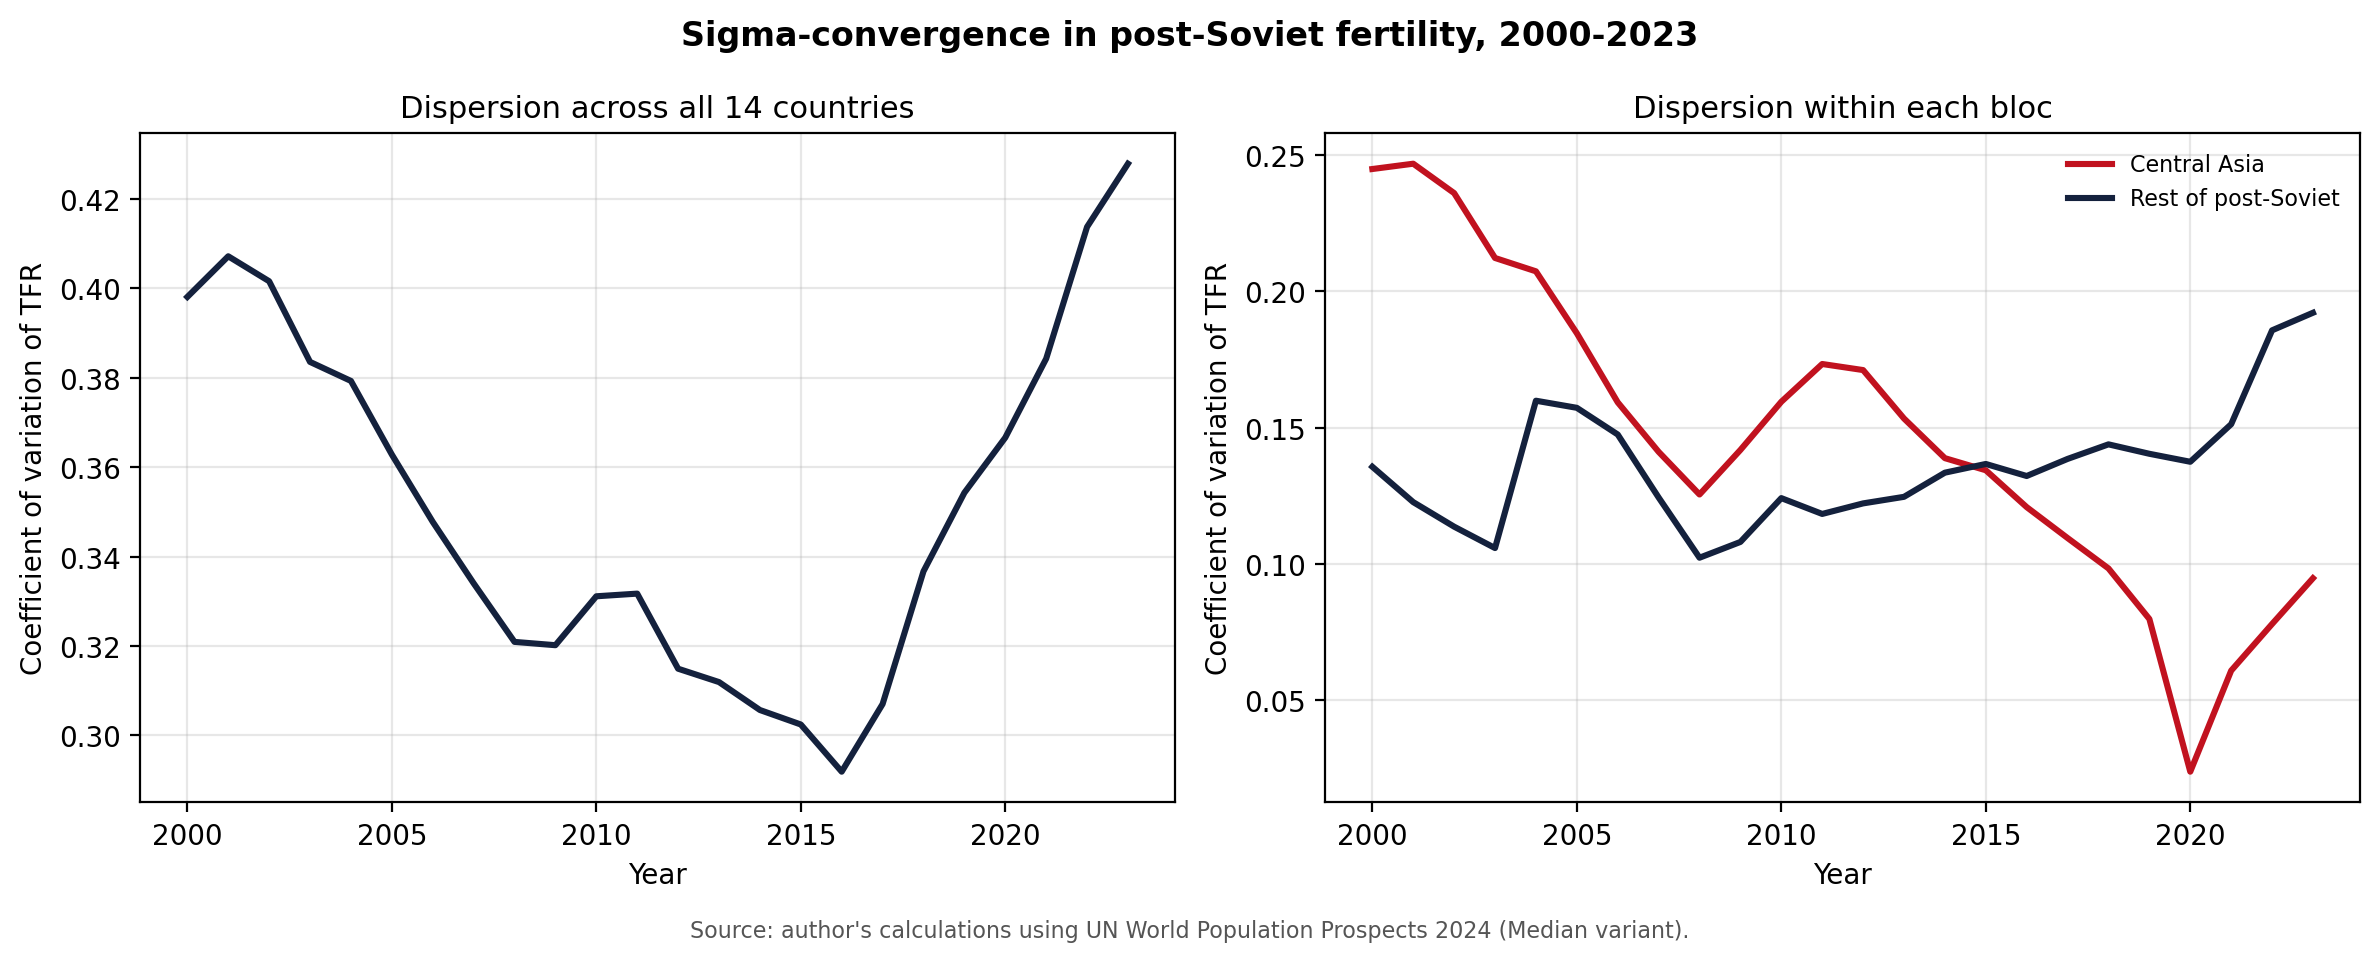
\includegraphics[width=\textwidth]{figures/fig5_sigma_convergence}
  \caption{$\sigma$-convergence in post-Soviet fertility. Left: dispersion across all fourteen countries. Right: dispersion within each bloc.}
  \label{fig:sigma}
\end{figure}

The second decomposition matters more. The right panel splits dispersion by bloc, and the two lines run in opposite directions. Within Central Asia, dispersion falls steeply and significantly, at $-0.0075$ per year ($p < 0.001$). Within the rest of the post-Soviet space it rises, at $+0.0016$ per year ($p = 0.025$). The four Central Asian countries have been growing more alike while the other ten have been growing less alike, and the pooled series in the left panel is simply these two movements cancelling.

Because the coefficient of variation is a ratio, a fall in it can reflect a rising mean rather than genuine compression. Here it does not. Central Asia's standard deviation fell from 0.653 in 2000 to 0.293 in 2023, and its interquartile range from 0.488 to 0.220; the comparison bloc's standard deviation rose from 0.187 to 0.278 and its interquartile range from 0.238 to 0.463. Both movements appear in absolute dispersion, not only in the scale-free measure, so neither is a denominator artefact. Note also that pooled absolute dispersion increased over the period (standard deviation 0.696 to 0.820) even though the pooled coefficient of variation barely moved, which is a further reminder that the ratio alone would have been misleading.

Two of these trends depend on particular countries and should be reported as such. Central Asia's internal convergence loses statistical significance when Tajikistan is dropped ($p = 0.132$), which makes sense: Tajikistan started highest and declined while the others rose, so it is doing much of the work of compressing the bloc. The comparison bloc's divergence loses significance when either Georgia ($p = 0.485$) or Ukraine ($p = 0.632$) is removed. These are country-sensitive patterns rather than group-wide regularities, and the leave-one-out results are given in full in Appendix~\ref{app:loo-convergence}.

The complementary test asks whether initially higher-fertility countries fell faster --- $\beta$-convergence. They did not. Estimating equation~\eqref{eq:beta} on the fourteen countries gives $\beta = +0.0013$ (HC3 standard error 0.0116, $p = 0.911$), with a confidence interval from $-0.024$ to $+0.027$ and an $R^2$ of 0.004. The point estimate is positive, meaning if anything that countries starting higher grew faster still, but it is indistinguishable from zero and the specification explains essentially none of the variation. Adding the Central Asia indicator raises $R^2$ to 0.270 without either coefficient reaching conventional significance (initial level $-0.020$, $p = 0.467$; Central Asia $+0.018$, $p = 0.368$). With fourteen observations this is a weak test, and the caution about regression to the mean noted in Section~\ref{sec:descriptive-methods} applies \parencite{quah1993}. What can be said is that the data offer no evidence of catch-up in either direction.

\subsection{The turning point after 2016}
\label{sec:turning-point}

Several of the results above locate a break at the same place. Pooled dispersion reaches its minimum in 2016 and rises thereafter. The bloc difference is at its narrowest in the same year. The comparison bloc's mean peaks in 2016 and declines from then on. Ten of the fourteen countries record their highest fertility in 2015 or later, which means the peak and the reversal are close together almost everywhere.

The single largest movement in the panel belongs to Uzbekistan, whose rate went from 2.57 in 2017 to 3.50 in 2023 --- an increase of 0.93 children per woman in six years, and the reason Uzbekistan holds the highest value in the sample by 2023 despite having been the second lowest of the four Central Asian countries in 2000. Kazakhstan's trajectory over the full window is almost as remarkable in a different way: from 1.90 in 2000, a level then comparable to Azerbaijan's, to 3.01 in 2023, a gain of 1.11 children per woman. These are not marginal adjustments to an existing regime.

At the other end, the declines after 2017 are broad and, in several countries, steep: Lithuania $-0.43$, Latvia $-0.36$, Belarus $-0.34$, Georgia $-0.33$, Ukraine $-0.32$, Azerbaijan $-0.29$. Nine of the ten countries outside Central Asia declined over these six years, Armenia being the single exception. Ukraine's fall is partly attributable to the full-scale invasion in 2022 and the displacement that followed, but the decline was underway before it: Ukraine had already dropped from 1.30 in 2017 to 1.15 by 2021.

It should be said clearly what this section does and does not establish. It documents a change in period fertility rates that is simultaneous across a large part of the sample and coincides with a visible break in dispersion. It does not identify what produced the break, and period rates cannot separate a genuine change in family size from a change in the timing of births \parencite{bongaarts1998}. That ten of fourteen countries peaked within a few years of each other is consistent with a common shift in the pace of postponement as much as with a common change in intended family size, and this analysis cannot tell the two apart.

\subsection{Are the descriptive results robust?}
\label{sec:desc-robust}

Two of the findings above --- the post-2016 rise in dispersion and the $\beta$ estimate --- depend on the end of the series, which is exactly where the World Population Prospects data are weakest, since eleven of the fourteen 2023 values are projections. Both are therefore recomputed on the two balanced sub-samples described in Section~\ref{sec:proj-check}.

The post-2016 dispersion slope is positive in all three samples: $+0.0195$ in the full sample, $+0.0237$ using all fourteen countries over 2000--2019 with no projected values anywhere, and $+0.0261$ using the ten countries with a non-projected observation in every year from 2017 to 2022. Rather than casting doubt on the divergence result, the exercise strengthens it: the finding is not an artefact of projected endpoints, and it is not an artefact of a shrinking, low-fertility-biased country set. The $\beta$ estimate is less stable --- $+0.0013$, $-0.0085$ and $+0.0052$ across the three samples --- but nothing rests on its sign, and all three are consistent with the conclusion that there is no detectable catch-up. Full results appear in Appendix~\ref{app:projection-check}.

\subsection{Summary}
\label{sec:trends-summary}

Fertility in the post-Soviet space did not converge between 2000 and 2023. The four Central Asian countries remained above the other ten in every single year, with no crossing at any point, and the difference between the two groups ended the period wider than it began. Underneath a flat pooled dispersion series, Central Asia converged internally while the rest of the region pulled apart. There is no evidence of catch-up: initially higher-fertility countries did not decline faster. And around 2016 the pattern changed, with a broad-based decline outside Central Asia accounting for roughly seventy per cent of a widening difference that reached 1.65 children per woman by 2023.

The remainder of the thesis takes that difference as its object. Chapter~\ref{sec:premium} asks how much of it moves together with observable economic conditions, and how much does not.

%  Requires: \input or \include of tables/tab_country_tfr.tex, and the
%  four PNG figures in figures/.
% =====================================================================

\section{Fertility Trends in the Post-Soviet Space, 2000--2023}
\label{sec:trends}

\subsection{Levels and trajectories}
\label{sec:levels}

In 2000 the fourteen countries in this study ranged from 1.11 children per woman in Ukraine to 3.49 in Tajikistan. Twenty-three years later the range had not narrowed. Ukraine had fallen to 0.98, one of the lowest national fertility rates ever recorded anywhere, while Uzbekistan had risen to 3.50. The endpoints are almost identical to where they started; what changed is which countries occupy them and how they got there.

\begin{table}[htbp]
\centering
\caption{Total fertility rate at selected dates, 2000--2023}
\label{tab:country-tfr}
\small
\begin{tabular}{lrrrrrr}
\toprule
 & 2000 & 2010 & 2017 & 2023 & $\Delta$ 2000--23 & $\Delta$ 2017--23 \\
\midrule
\multicolumn{7}{l}{\textit{Central Asia}} \\
\quad Kazakhstan & 1.90 & 2.61 & 2.75 & 3.01 & +1.11 & +0.27 \\
\quad Kyrgyzstan & 2.58 & 3.10 & 3.04 & 2.80 & +0.22 & -0.24 \\
\quad Tajikistan & 3.49 & 3.46 & 3.29 & 3.07 & -0.42 & -0.22 \\
\quad Uzbekistan & 2.70 & 2.44 & 2.57 & 3.50 & +0.80 & +0.93 \\
\addlinespace
\quad \textit{Bloc mean} & 2.67 & 2.90 & 2.91 & 3.10 & +0.43 & +0.18 \\
\addlinespace
\multicolumn{7}{l}{\textit{Rest of post-Soviet space}} \\
\quad Armenia & 1.47 & 1.59 & 1.56 & 1.71 & +0.24 & +0.15 \\
\quad Azerbaijan & 1.70 & 1.92 & 1.96 & 1.67 & -0.03 & -0.29 \\
\quad Belarus & 1.27 & 1.48 & 1.55 & 1.21 & -0.06 & -0.34 \\
\quad Estonia & 1.35 & 1.72 & 1.60 & 1.35 & +0.00 & -0.25 \\
\quad Georgia & 1.61 & 1.97 & 2.14 & 1.81 & +0.20 & -0.33 \\
\quad Latvia & 1.24 & 1.37 & 1.70 & 1.34 & +0.09 & -0.36 \\
\quad Lithuania & 1.38 & 1.50 & 1.63 & 1.20 & -0.18 & -0.43 \\
\quad Moldova & 1.50 & 1.70 & 1.81 & 1.73 & +0.23 & -0.08 \\
\quad Russia & 1.19 & 1.59 & 1.63 & 1.45 & +0.26 & -0.18 \\
\quad Ukraine & 1.11 & 1.44 & 1.30 & 0.98 & -0.13 & -0.32 \\
\addlinespace
\quad \textit{Bloc mean} & 1.38 & 1.63 & 1.69 & 1.44 & +0.06 & -0.24 \\
\addlinespace
\midrule
\multicolumn{7}{l}{Difference in bloc means} \\
\quad Central Asia $-$ rest & 1.28 & 1.27 & 1.23 & 1.65 & & \\
\bottomrule
\end{tabular}

\begin{minipage}{\textwidth}\footnotesize
\vspace{4pt}
\emph{Source:} UN World Population Prospects 2024, median variant; author's calculations.
\emph{Note:} Bloc means and differences are computed from unrounded country values,
so they need not equal the difference of the rounded figures shown. Eleven of the
fourteen 2023 values are WPP projections rather than retrospective interpolated
estimates; only Latvia, Lithuania and Russia are interpolated in 2023.
\end{minipage}
\end{table}

Table~\ref{tab:country-tfr} sets out the individual trajectories, and Figure~\ref{fig:all-countries} shows all fourteen together. Two things stand out immediately. The first is the separation. In every single year of the panel, the lowest-fertility Central Asian country lies above the highest-fertility country outside Central Asia. There is not one crossing in twenty-four years, and the narrowest the two groups ever come is 0.195 children per woman, in 2012.

\begin{figure}[htbp]
  \centering
  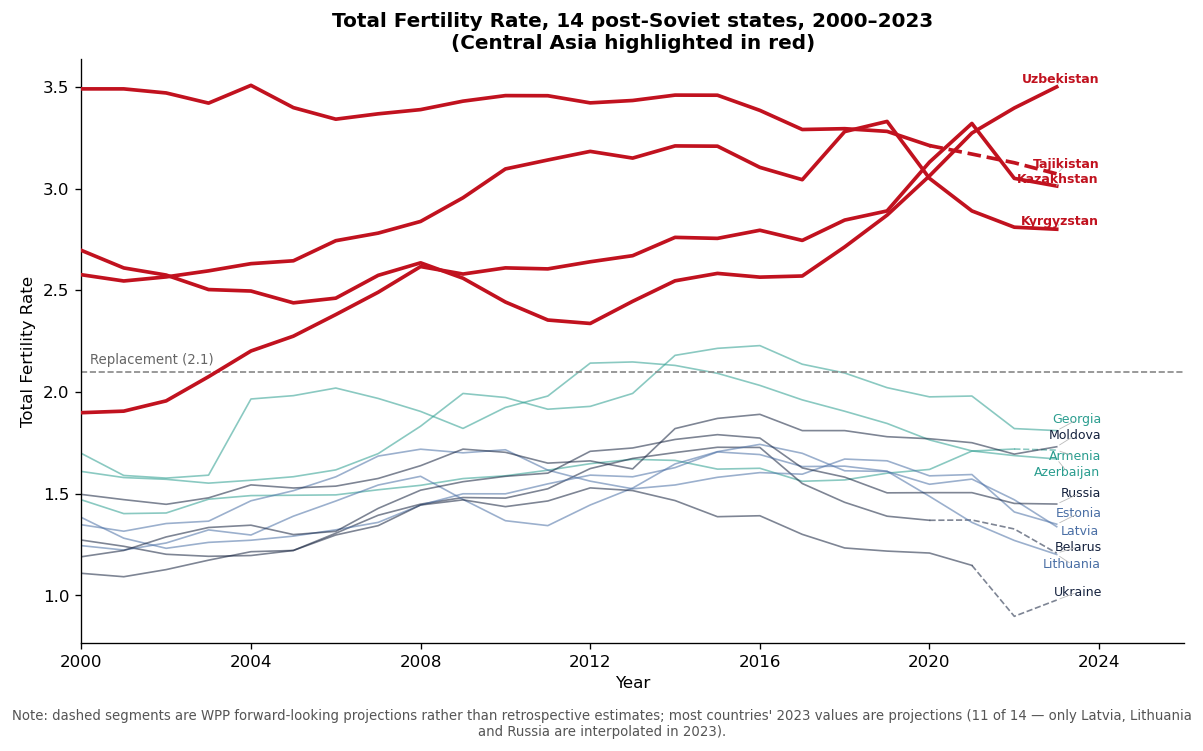
\includegraphics[width=\textwidth]{figures/fig1_all_countries}
  \caption{Total fertility rate, fourteen post-Soviet states, 2000--2023. Central Asian countries in red. Dashed segments are WPP forward-looking projections rather than retrospective estimates.}
  \label{fig:all-countries}
\end{figure}

The second is that the separation does not come from a shared decline at different speeds. Most of the sample rose for the first fifteen years or so. Ten of the fourteen countries recorded their highest fertility of the period in 2015 or later, and only Tajikistan among the Central Asian states peaked early, in 2004. Russia's rate climbed from 1.19 to a high of 1.79 in 2015 before falling back; Latvia went from 1.24 to 1.74 in 2016; Georgia reached 2.23 in 2016, briefly above replacement. This broad recovery from the post-Soviet trough is well documented for the European successor states \parencite{billingsley2010,grigoras2019} and for Central Asia \parencite{spoorenberg2015}. What has not been documented, because the comparative literature ends before it, is what happened after that.

By 2023 ten of the fourteen countries were below the replacement level of 2.1, and the four that were not are the four Central Asian states. Three of the ten European and Caucasian countries had fallen below 1.25.

\subsection{The difference between the blocs}
\label{sec:gap}

Figure~\ref{fig:bloc-means} tracks the two bloc means with the country range around each. The Central Asian mean rose from 2.67 in 2000 to 3.09 in 2023, an increase of 0.43 children per woman. The rest of the post-Soviet space rose too, from 1.38 to a peak of 1.77 in 2016, and then gave nearly all of it back, ending at 1.44.

\begin{figure}[htbp]
  \centering
  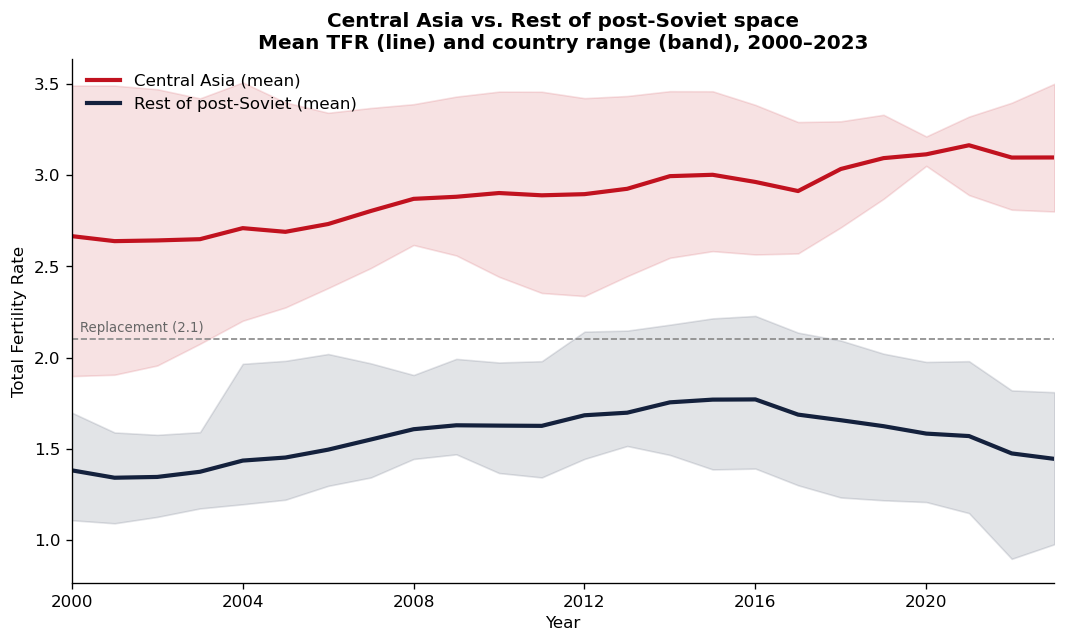
\includegraphics[width=0.92\textwidth]{figures/fig2_bloc_means}
  \caption{Mean total fertility rate by bloc, with the country range shown as a shaded band, 2000--2023.}
  \label{fig:bloc-means}
\end{figure}

The difference between the two means is the central descriptive object of this thesis, and its behaviour over time is more interesting than its average size. Figure~\ref{fig:gap} plots it year by year. From 2000 to 2016 it is remarkably flat, moving within a narrow corridor between 1.19 and 1.30 and drifting very slightly downward. Then it changes character: 1.19 in 2016, 1.38 in 2018, 1.53 in 2020, 1.65 in 2023. Over seven years it widened by 0.46 children per woman, having barely moved in the previous sixteen.

\begin{figure}[htbp]
  \centering
  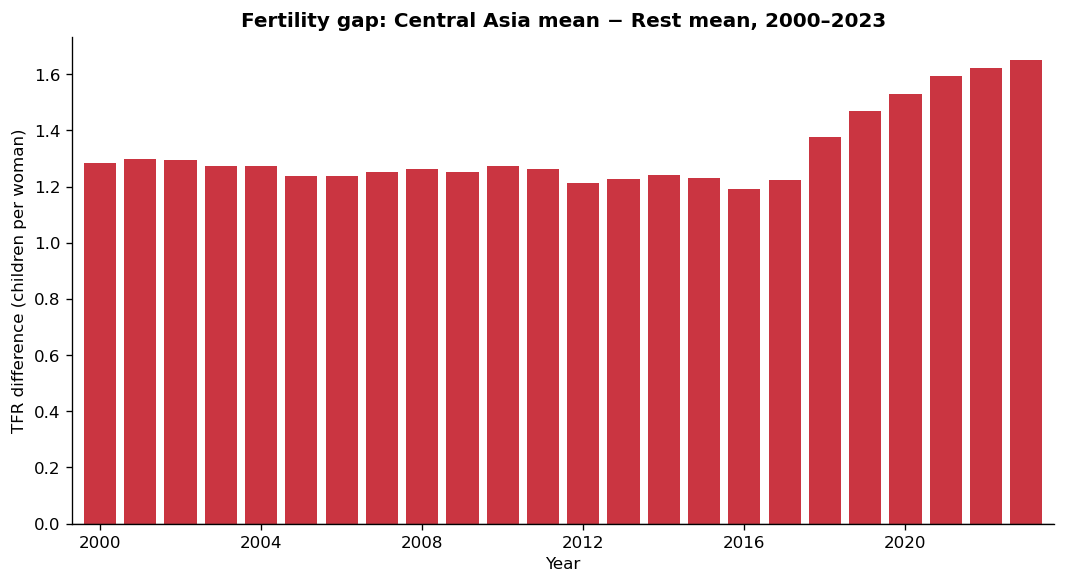
\includegraphics[width=0.88\textwidth]{figures/fig4_gap}
  \caption{Difference between Central Asian and other post-Soviet mean total fertility rates, 2000--2023.}
  \label{fig:gap}
\end{figure}

It is worth being precise about where that widening came from, because the intuitive reading is misleading. Central Asia did rise after 2016, by 0.13 children per woman. But the comparison bloc fell by 0.33 over the same years. Of the total widening of 0.46, roughly seventy per cent is the rest of the post-Soviet space declining and only thirty per cent is Central Asia climbing. The divergence is therefore as much a story about Ukraine, Lithuania, Latvia and Belarus as it is about Uzbekistan, and any account that treats it purely as a Central Asian phenomenon is describing less than a third of the movement.

Disaggregating the comparison bloc confirms that the decline is broad rather than driven by one sub-region. Between 2016 and 2023 the Baltic mean fell from 1.68 to 1.30, the Eastern European mean from 1.70 to 1.34, and the Caucasus mean from 1.96 to 1.73. All three moved in the same direction over the same years. The Caucasus remains the intermediate case throughout, sitting consistently above the Baltic and Eastern European groups and well below Central Asia, which is what one would expect of a region that shares some of Central Asia's cultural and nuptiality characteristics without sharing all of them. The sub-group series are reported in Appendix~\ref{app:subgroups}.

\subsection{Convergence and divergence}
\label{sec:convergence}

If the post-Soviet states had been converging on a common fertility regime, dispersion across them should have fallen. The standard way to test this is $\sigma$-convergence: the coefficient of variation of fertility computed across countries within each year.

Taken over the full window, the answer looks like nothing happened. The coefficient of variation was 0.398 in 2000 and 0.428 in 2023, and a linear trend through the whole series gives a slope of $-0.0007$ per year with a p-value of 0.758. Read on its own, that says the fourteen countries were no more alike at the end than at the beginning.

That reading is wrong in an instructive way, because the flat trend is the average of two things moving in opposite directions. The left panel of Figure~\ref{fig:sigma} shows the pooled series falling steadily from 2000 to a minimum of 0.292 in 2016, then rising sharply to 0.428 by 2023. Fitted separately, the two phases give slopes of $-0.0072$ per year over 2000--2016 ($p < 0.001$) and $+0.0195$ per year afterwards. The second figure carries no p-value: seven annual observations are not enough for reliable inference on a serially correlated series, so only the sign and the visible pattern are claimed. The post-2016 window is short, but the direction is unambiguous and, as Section~\ref{sec:desc-robust} shows, it survives every check applied to it.

\begin{figure}[htbp]
  \centering
  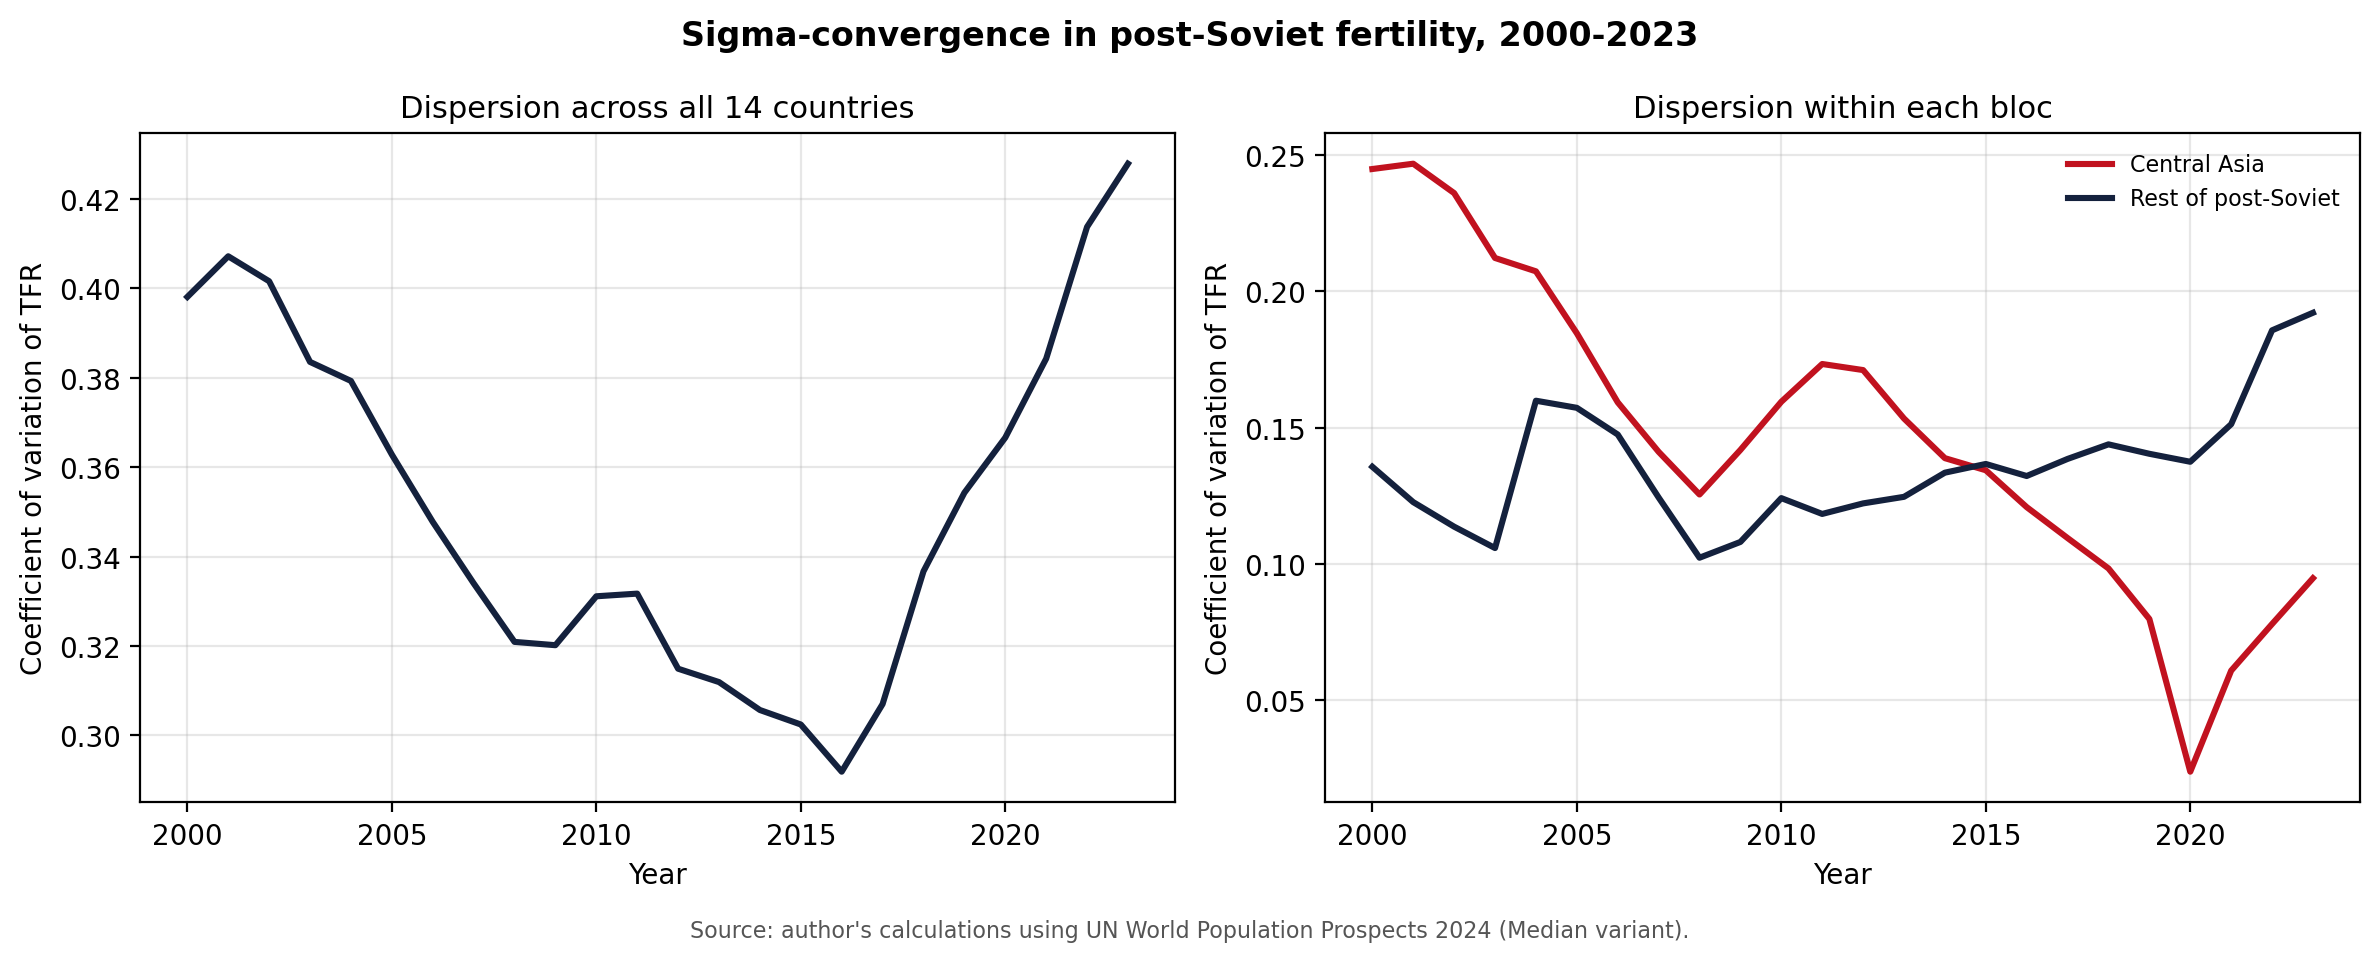
\includegraphics[width=\textwidth]{figures/fig5_sigma_convergence}
  \caption{$\sigma$-convergence in post-Soviet fertility. Left: dispersion across all fourteen countries. Right: dispersion within each bloc.}
  \label{fig:sigma}
\end{figure}

The second decomposition matters more. The right panel splits dispersion by bloc, and the two lines run in opposite directions. Within Central Asia, dispersion falls steeply and significantly, at $-0.0075$ per year ($p < 0.001$). Within the rest of the post-Soviet space it rises, at $+0.0016$ per year ($p = 0.025$). The four Central Asian countries have been growing more alike while the other ten have been growing less alike, and the pooled series in the left panel is simply these two movements cancelling.

Because the coefficient of variation is a ratio, a fall in it can reflect a rising mean rather than genuine compression. Here it does not. Central Asia's standard deviation fell from 0.653 in 2000 to 0.293 in 2023, and its interquartile range from 0.488 to 0.220; the comparison bloc's standard deviation rose from 0.187 to 0.278 and its interquartile range from 0.238 to 0.463. Both movements appear in absolute dispersion, not only in the scale-free measure, so neither is a denominator artefact. Note also that pooled absolute dispersion increased over the period (standard deviation 0.696 to 0.820) even though the pooled coefficient of variation barely moved, which is a further reminder that the ratio alone would have been misleading.

Two of these trends depend on particular countries and should be reported as such. Central Asia's internal convergence loses statistical significance when Tajikistan is dropped ($p = 0.132$), which makes sense: Tajikistan started highest and declined while the others rose, so it is doing much of the work of compressing the bloc. The comparison bloc's divergence loses significance when either Georgia ($p = 0.485$) or Ukraine ($p = 0.632$) is removed. These are country-sensitive patterns rather than group-wide regularities, and the leave-one-out results are given in full in Appendix~\ref{app:loo-convergence}.

The complementary test asks whether initially higher-fertility countries fell faster --- $\beta$-convergence. They did not. Estimating equation~\eqref{eq:beta} on the fourteen countries gives $\beta = +0.0013$ (HC3 standard error 0.0116, $p = 0.911$), with a confidence interval from $-0.024$ to $+0.027$ and an $R^2$ of 0.004. The point estimate is positive, meaning if anything that countries starting higher grew faster still, but it is indistinguishable from zero and the specification explains essentially none of the variation. Adding the Central Asia indicator raises $R^2$ to 0.270 without either coefficient reaching conventional significance (initial level $-0.020$, $p = 0.467$; Central Asia $+0.018$, $p = 0.368$). With fourteen observations this is a weak test, and the caution about regression to the mean noted in Section~\ref{sec:descriptive-methods} applies \parencite{quah1993}. What can be said is that the data offer no evidence of catch-up in either direction.

\subsection{The turning point after 2016}
\label{sec:turning-point}

Several of the results above locate a break at the same place. Pooled dispersion reaches its minimum in 2016 and rises thereafter. The bloc difference is at its narrowest in the same year. The comparison bloc's mean peaks in 2016 and declines from then on. Ten of the fourteen countries record their highest fertility in 2015 or later, which means the peak and the reversal are close together almost everywhere.

The single largest movement in the panel belongs to Uzbekistan, whose rate went from 2.57 in 2017 to 3.50 in 2023 --- an increase of 0.93 children per woman in six years, and the reason Uzbekistan holds the highest value in the sample by 2023 despite having been the second lowest of the four Central Asian countries in 2000. Kazakhstan's trajectory over the full window is almost as remarkable in a different way: from 1.90 in 2000, a level then comparable to Azerbaijan's, to 3.01 in 2023, a gain of 1.11 children per woman. These are not marginal adjustments to an existing regime.

At the other end, the declines after 2017 are broad and, in several countries, steep: Lithuania $-0.43$, Latvia $-0.36$, Belarus $-0.34$, Georgia $-0.33$, Ukraine $-0.32$, Azerbaijan $-0.29$. Nine of the ten countries outside Central Asia declined over these six years, Armenia being the single exception. Ukraine's fall is partly attributable to the full-scale invasion in 2022 and the displacement that followed, but the decline was underway before it: Ukraine had already dropped from 1.30 in 2017 to 1.15 by 2021.

It should be said clearly what this section does and does not establish. It documents a change in period fertility rates that is simultaneous across a large part of the sample and coincides with a visible break in dispersion. It does not identify what produced the break, and period rates cannot separate a genuine change in family size from a change in the timing of births \parencite{bongaarts1998}. That ten of fourteen countries peaked within a few years of each other is consistent with a common shift in the pace of postponement as much as with a common change in intended family size, and this analysis cannot tell the two apart.

\subsection{Are the descriptive results robust?}
\label{sec:desc-robust}

Two of the findings above --- the post-2016 rise in dispersion and the $\beta$ estimate --- depend on the end of the series, which is exactly where the World Population Prospects data are weakest, since eleven of the fourteen 2023 values are projections. Both are therefore recomputed on the two balanced sub-samples described in Section~\ref{sec:proj-check}.

The post-2016 dispersion slope is positive in all three samples: $+0.0195$ in the full sample, $+0.0237$ using all fourteen countries over 2000--2019 with no projected values anywhere, and $+0.0261$ using the ten countries with a non-projected observation in every year from 2017 to 2022. Rather than casting doubt on the divergence result, the exercise strengthens it: the finding is not an artefact of projected endpoints, and it is not an artefact of a shrinking, low-fertility-biased country set. The $\beta$ estimate is less stable --- $+0.0013$, $-0.0085$ and $+0.0052$ across the three samples --- but nothing rests on its sign, and all three are consistent with the conclusion that there is no detectable catch-up. Full results appear in Appendix~\ref{app:projection-check}.

\subsection{Summary}
\label{sec:trends-summary}

Fertility in the post-Soviet space did not converge between 2000 and 2023. The four Central Asian countries remained above the other ten in every single year, with no crossing at any point, and the difference between the two groups ended the period wider than it began. Underneath a flat pooled dispersion series, Central Asia converged internally while the rest of the region pulled apart. There is no evidence of catch-up: initially higher-fertility countries did not decline faster. And around 2016 the pattern changed, with a broad-based decline outside Central Asia accounting for roughly seventy per cent of a widening difference that reached 1.65 children per woman by 2023.

The remainder of the thesis takes that difference as its object. Chapter~\ref{sec:premium} asks how much of it moves together with observable economic conditions, and how much does not.
